\chapter{Trends with Black Hole Properties} \label{BH}
 
In Chapter~\ref{SEDs} we explored the multi-wavelength quasar SEDs as the functions of various properties, but we did not consider them as a function of $\mbh$ or accretion rate, as those quantities are determined more indirectly than the properties in Chapter~\ref{SEDs}.  The analysis of Chapter~\ref{Dust} was restricted to optical--UV photometry and SDSS spectroscopy since that is where dust extinction has the largest effect.  Here we extend the analysis of Chapter~\ref{Dust} to the full mid-IR--X-ray SEDs and the analysis of Chapter~\ref{SEDs} to the $\mbh$ and $\dot{M}_{\rm BH}$ distributions.
%In Chapter~\ref{SEDs} we did not consider the SEDs as a function of $\mbh$ or accretion rate as those quantities are determined more indirectly than the properties in Chapter~\ref{SEDs}.  
%To determine these quantities we must first correct the individual quasar SEDs from Chapter~\ref{SEDs} for the dust extinction that was quantified in Chapter~\ref{Dust}. 
%In this chapter we aim to correct the individual quasar SEDs from Chapter~\ref{SEDs} for the dust extinction that was quantified in Chapter~\ref{Dust}.  
%Applying this correction allows for the calculation of more accurate bolometric luminosities (\lbol) and in turn more accurate accretions rates. With these updated \lbol\ values we explore the dependency of the bolometric correction (\bctwofive) on a quasar's intrinsic color and associated extinction.  
In \S\ref{dust_seds} we construct mean SEDs as a functions of the quasars' intrinsic colors and $\ebv$ and correct them for dust extinction.
Using the $\mbh$ sample presented in \S\ref{BH_data}, \S\ref{mbh_seds} explores how a quasar's SED and \bctwofive\ change as functions of $\mbh$ and the Eddington ratio ($\lf$; a proxy for $\dot{M}_{BH}$).   Finally we conclude in \S\ref{BH_conclusions}.
%In \S\ref{mbh_seds} we looks for trends in mean SEDs based on $\mbh$ and the $\lf$ and

\section{Dust Corrected Mean SEDs} \label{dust_seds}

In \S\ref{sec:mcmc_results} we showed that our quasars span a range of intrinsic colors and $\ebv$ values.  
In particular, our sample was split over a 10x10 grid in the parameter space span by $\ebv$ and 2.5$\dal$\footnote{$\dal = \alpha_{\lambda, {\rm  mode}} - \alpha_\lambda$ (see \S\ref{sec:red_v_red:phot})}.
Given the uncertainties in the measurements of these quantities, this binning is weighted by the probability of a particular quasar belonging to any given bin (see \S\ref{sec:spectra} for more details).  Using these bins and weights we will now extend the composite optical spectra to mean SEDs.
% have constructed mean SEDs as a function of both dust extinction and intrinsic color.

These mean SEDs were constructed in the same manner as the subsamples in \S\ref{sed}: the observed data were shifted to the rest frame, placed on a common grid in $\log{(\nu)}$, missing data were gap-filled, and kriging was used to interpolate the data onto the rest of the grid.  The SEDs were initially gap-filled using the mid-luminosity mean SED from \S\ref{Luminosity SED} and mean SEDs were made for each bin in color--$\ebv$ space.  To ensure the gap-filling is based on the observed properties of the quasars within each bin and not on the gap-filling model chosen, the resulting mean SEDs in each bin were used to gap-fill their respective bin.  This process was repeated for 10 iterations, after which the mean SEDs did not change significantly.
%The resulting mean SEDs were used for gap filling, and this process was repeated for 10 iterations to make sure any trends seen within each bin were a result of the data and not the gap filling model.

\begin{figure}[t]
\begin{center}
\begin{tabular}{cc}
	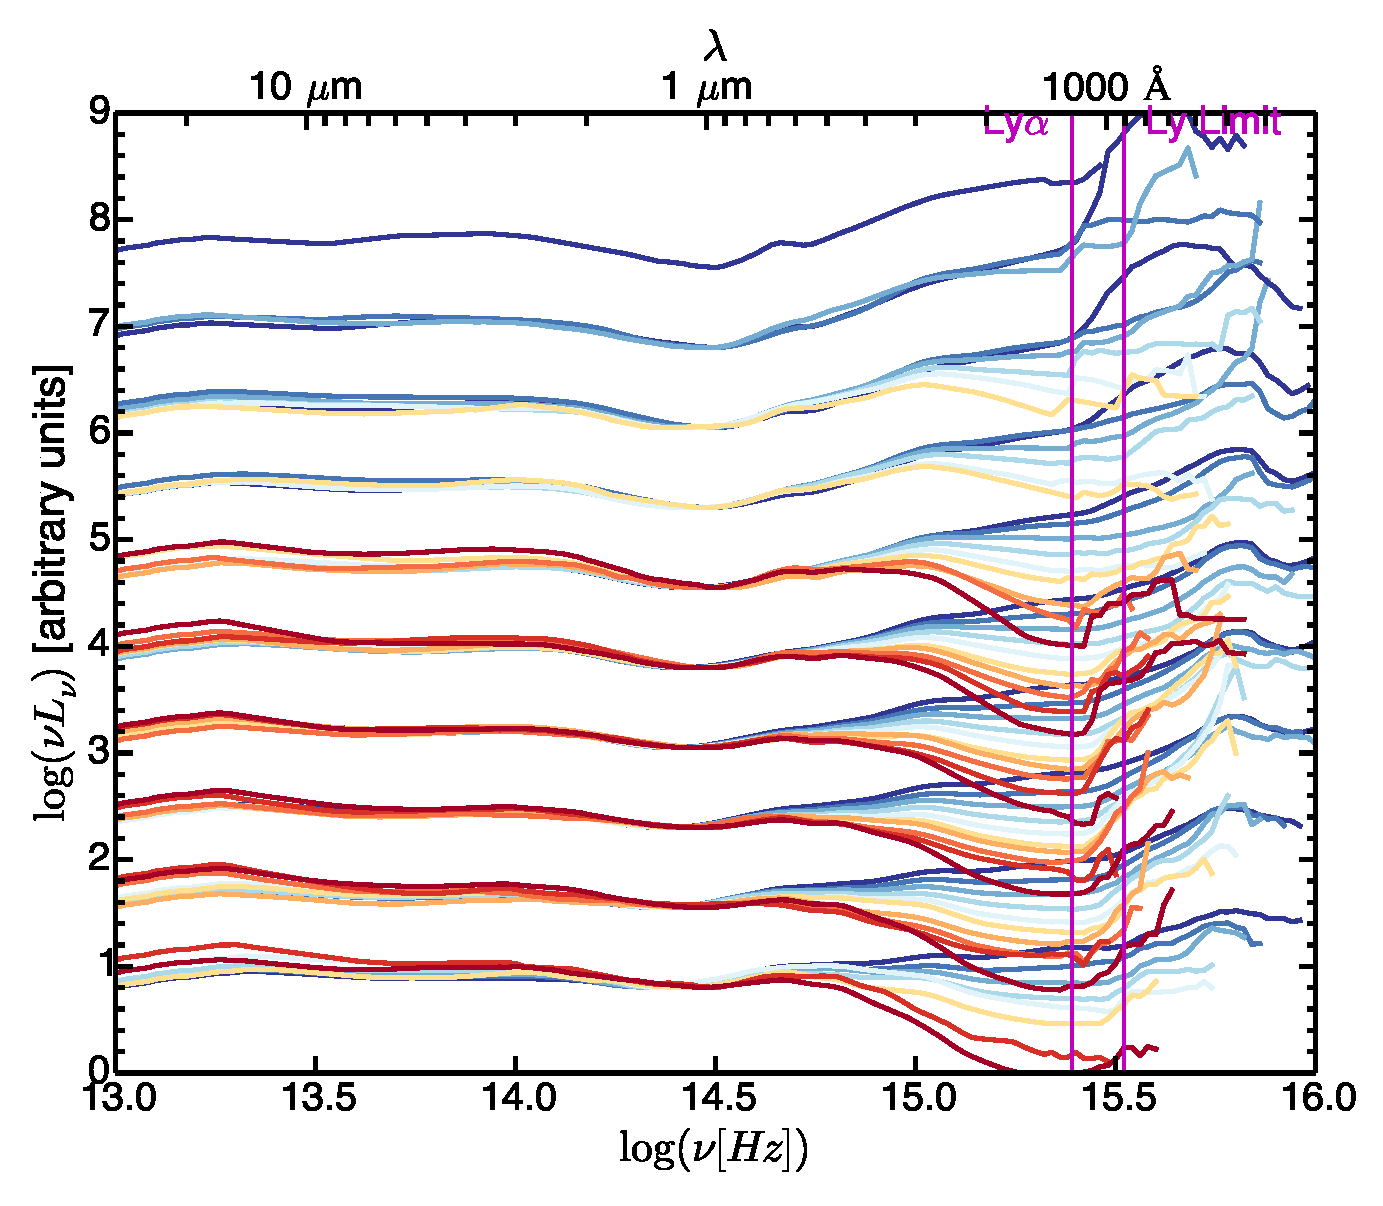
\includegraphics[width=4in]{images/BH/f3a} & 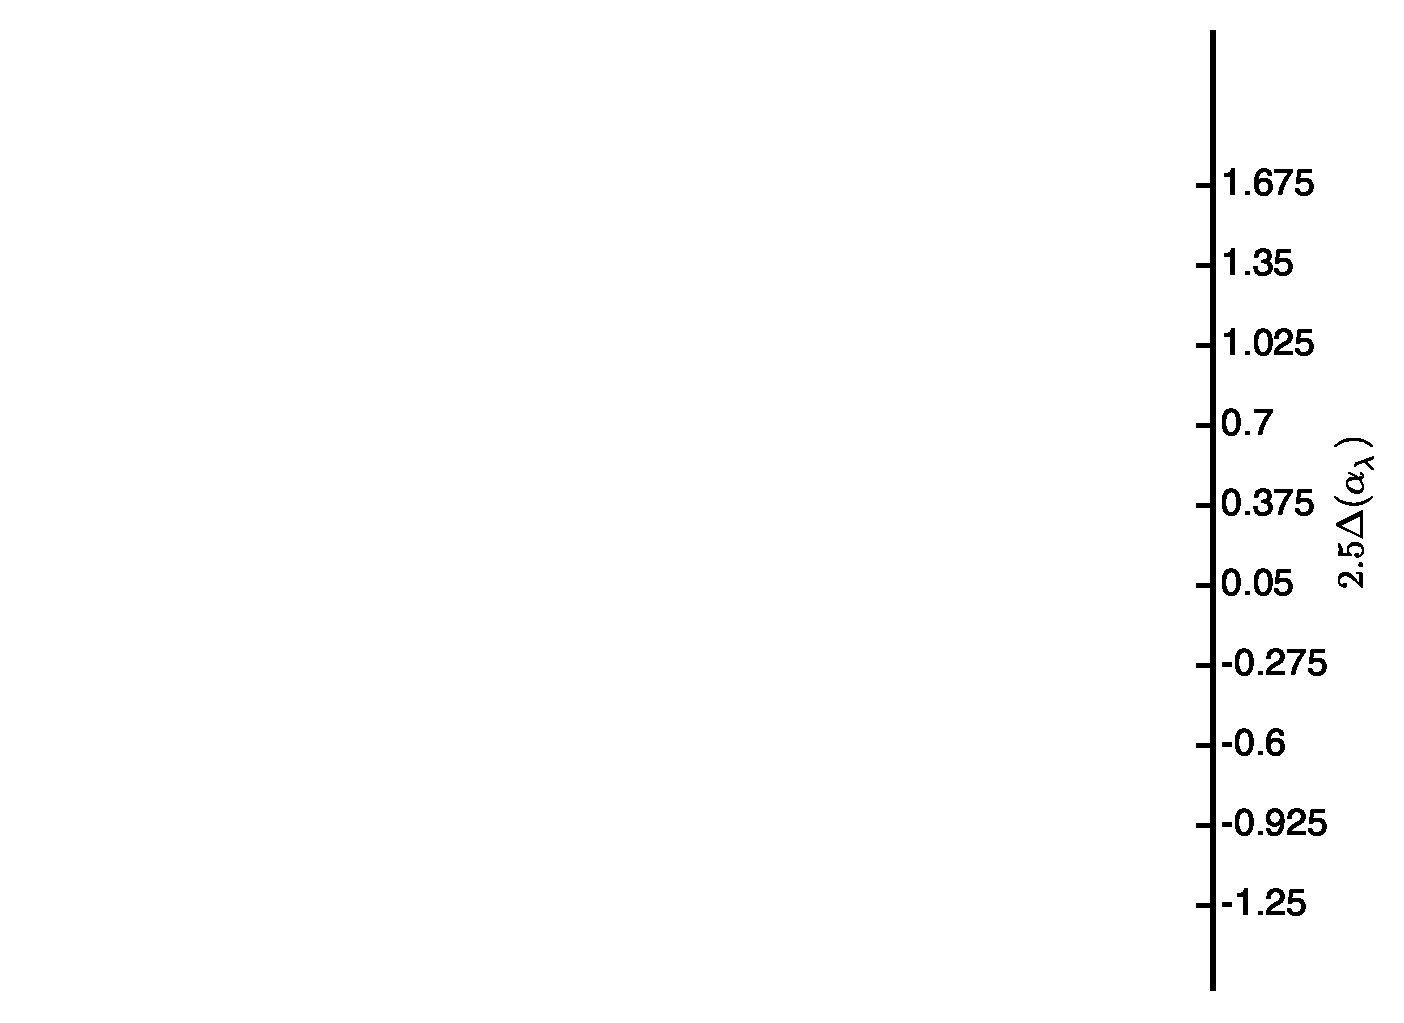
\includegraphics[trim={7.8in -.65in 0 0}, clip=true, height=3.25in]{images/BH/alpha_ticks}\\
	\hspace{.4cm} 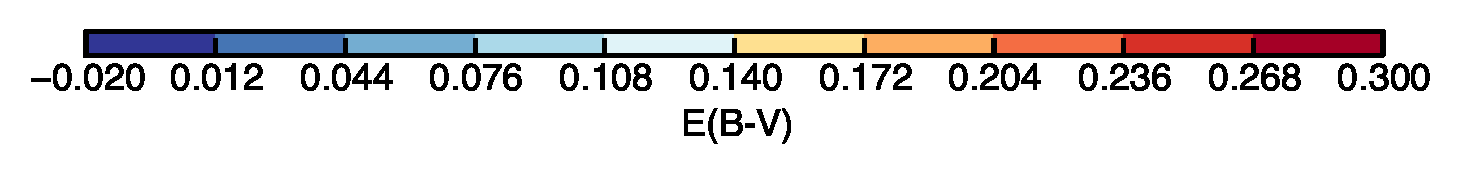
\includegraphics[width=3.75in]{images/BH/ebv_colorbar} &
\end{tabular}
\caption[Mean SEDs grouped by color]{\label{sed_dust} Mean SEDs for quasars grouped by intrinsic color with the intrinsically bluest quasars on top and the intrinsically reddest quasars on the bottom.  The colors indicate the $\ebv$ for each SED and the vertical magenta lines indicate the Ly$\alpha$ and Ly Limit for reference.  As seen in Chapter~\ref{Dust}, there are very few blue quasars with heavy reddening.  
%In the mid-IR the spectral index between 7--11\,$\mu$m becomes redder for the quasars with more dust extinction. 
All SEDs have been normalized at their minimum value near \onemum, and each grouping has been offset vertically for clarity.}
\end{center}
\end{figure}

\begin{figure}[t]
\begin{center}
\begin{tabular}{cc}
	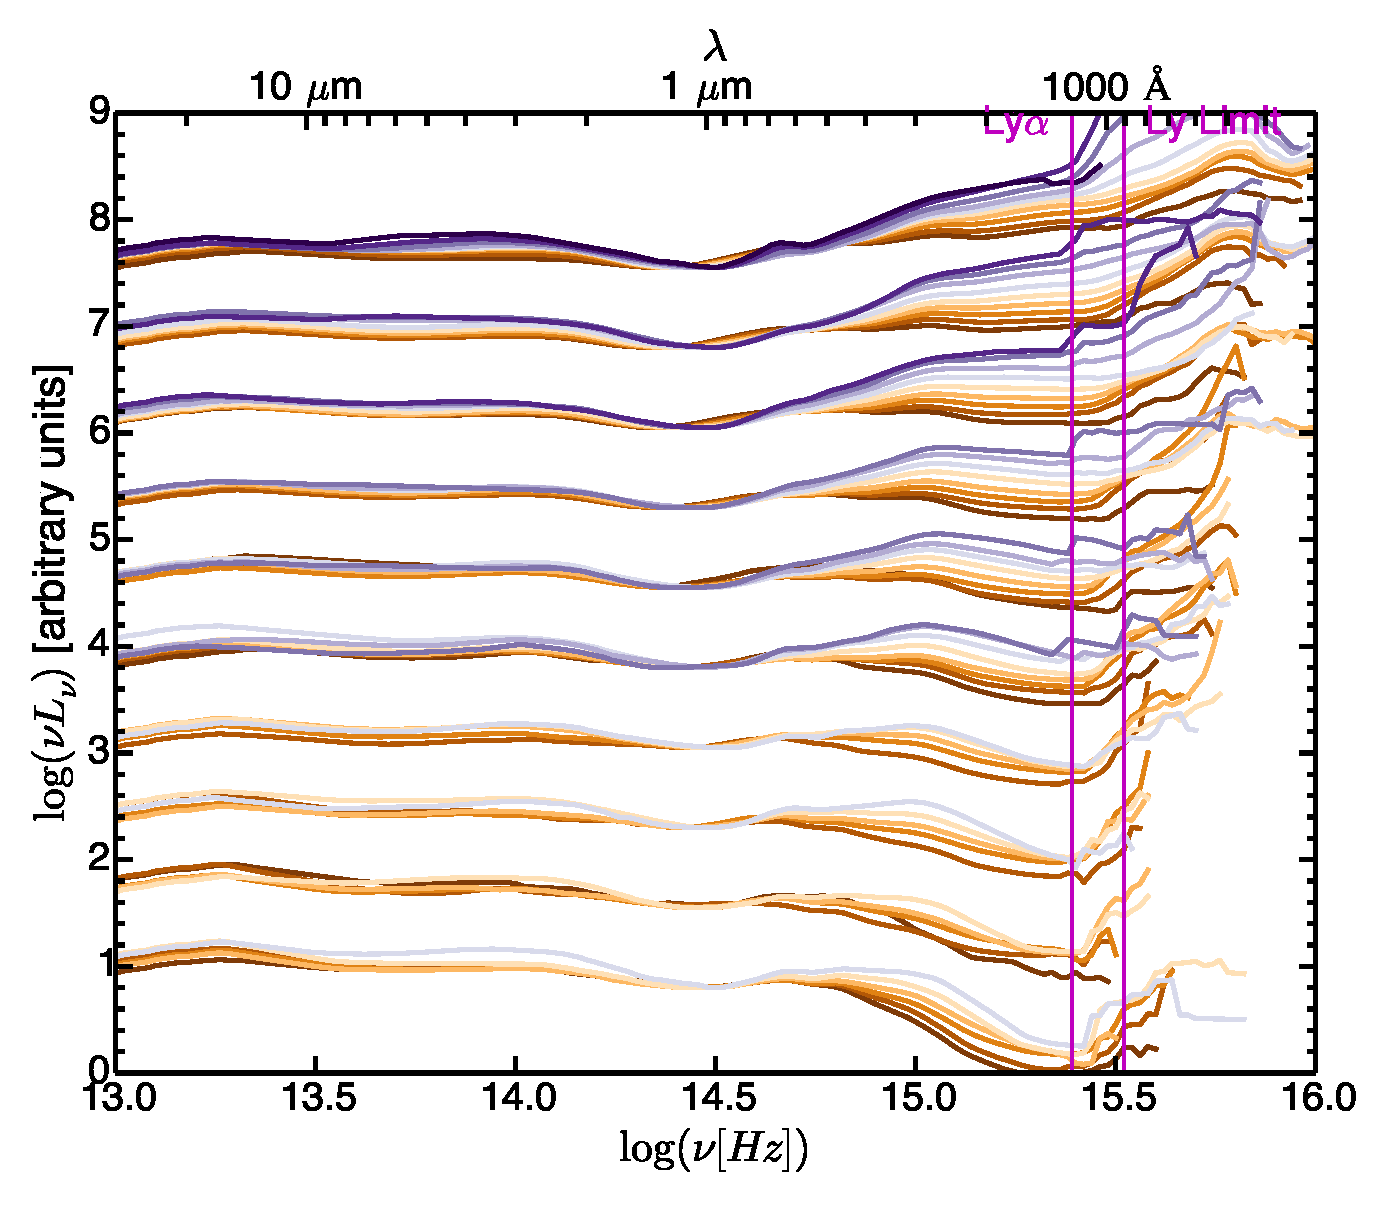
\includegraphics[width=4in]{images/BH/f3b} & 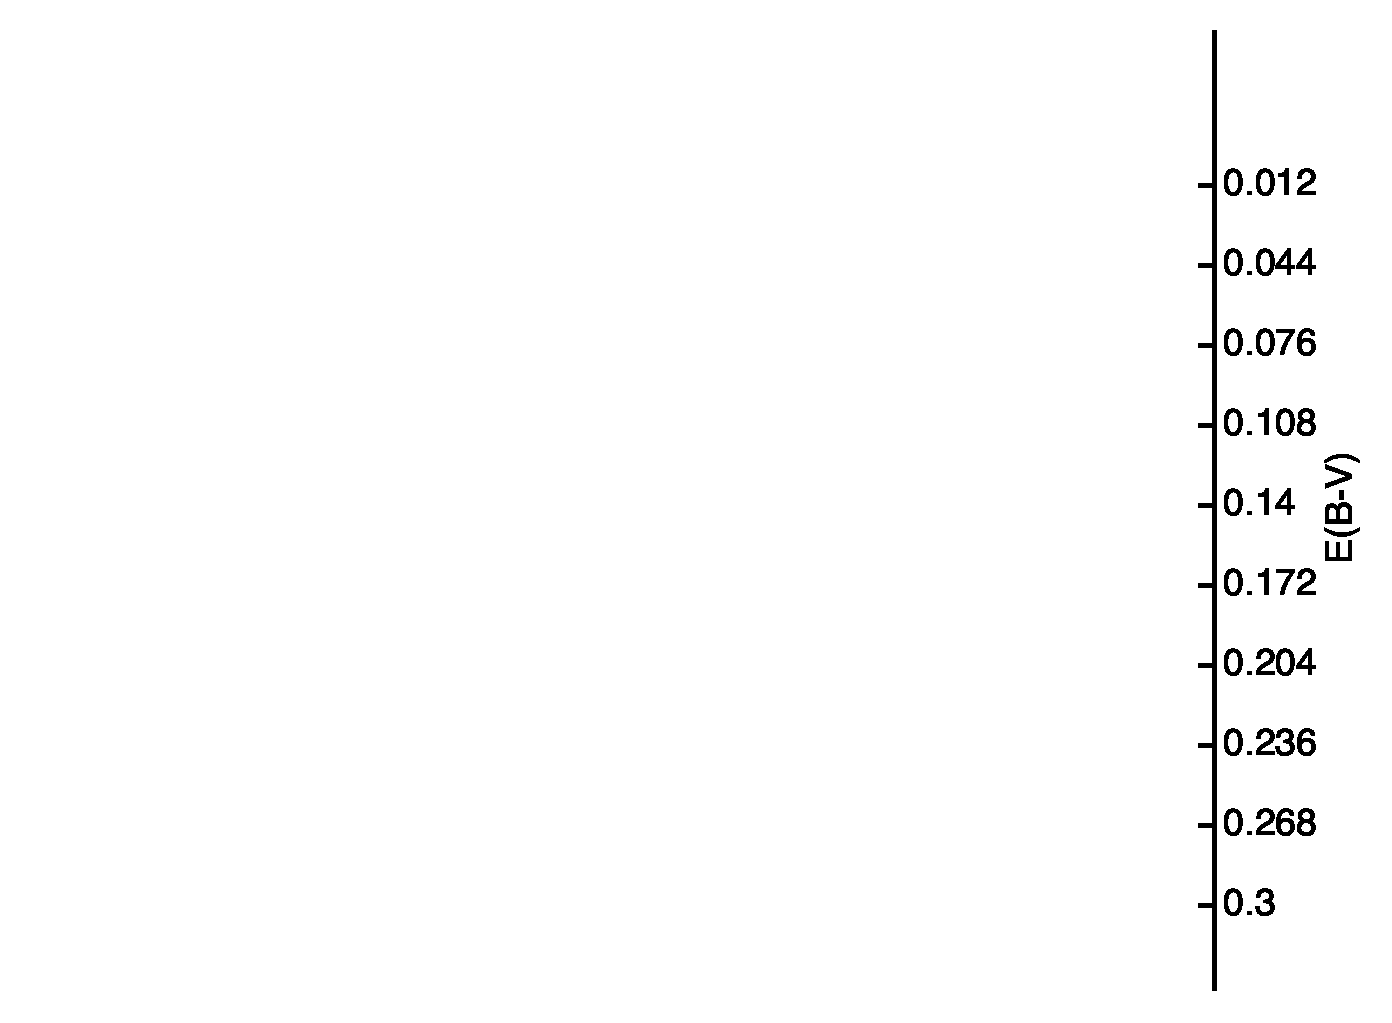
\includegraphics[trim={7.8in -.65in 0 0}, clip=true, height=3.25in]{images/BH/ebv_ticks}\\
	\hspace{.4cm} 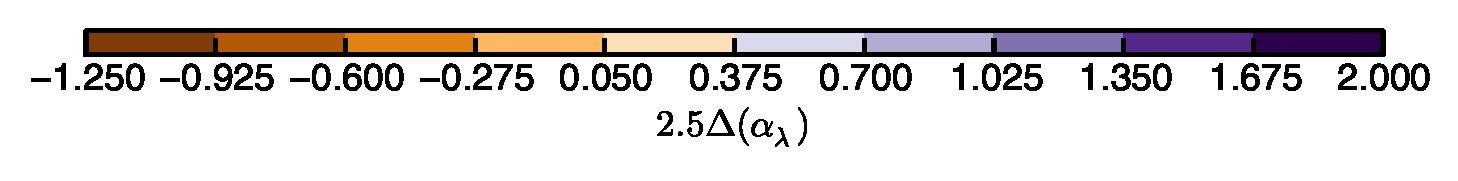
\includegraphics[width=3.75in]{images/BH/alpha_colorbar} &
\end{tabular}
\caption[Mean SEDs grouped by dust]{\label{sed_color} The same SEDs from Figure~\ref{sed_dust} grouped by $\ebv$ with least reddened quasar on top and the most reddened quasars on the bottom. The colors indicate the intrinsic color for each SED and the vertical magenta lines indicate the Ly$\alpha$ and Ly Limit for reference. There is a clear trend in the mid-IR with the blue quasars having more hot dust than the red quasars.  The blue quasars also show a residual flux in the H$\alpha$ line (6563\,\AA).  All SEDs have been normalized at their minimum value near \onemum, and each grouping has been offset vertically for clarity.}
\end{center}
\end{figure}

To get an idea of how large of an effect the dust corrections have, we present the SEDs as a function of color and reddening both before and after dust correction.  Since we will be using estimates of $\mbh$ later in our analysis, we restrict our sample to the non-BAL quasars from Chapter~\ref{Dust}.
Figure~\ref{sed_dust} shows the resulting SEDs for each bin grouped by common intrinsic color before applying the extinction correction. Unlike Figure~\ref{fig:spec}, here we are showing the full SED from the multi-wavelength photometry (as in Chapter~\ref{SEDs}) and not the composite spectra. To highlight differences in the mid-IR and optical regions, each mean SED has been normalized at the minimum value of their dip near \onemum.  As seen in Chapter~\ref{Dust}, there are very few non-BAL blue quasars with heavy reddening (see left panel of Figure~\ref{fig:indv_fits_SMC}). The clearest trend in these SEDs is the change in the optical--UV region where the SEDs with more dust extinction show more curvature than the SEDs with no extinction.  There is also a slight trend in the mid-IR where the spectral index between 7--11\,$\mu$m becomes redder for the quasars with more dust extinction.

Figure~\ref{sed_color} takes the same SEDs from Figure~\ref{sed_dust} but groups the SEDs by common $\ebv$. When grouped in this manner, there is a clear trend in the mid-IR where the intrinsically blue quasars have more hot dust emission than intrinsically red ones.  This is similar to the trend seen in the high luminosity quasars from \S\ref{Luminosity SED} and the high luminosity quasars from \citet{Gallagher:2007a}. Additionally, the bluer quasars show more residual\footnote{In \S\ref{sec:emission} we remove the mean contribution of spectral lines in the SEDs.} H$\alpha$ emission (6563\,\AA), consistent with the stacked spectra from \S\ref{sec:spectra}.

The top group of Figure~\ref{sed_color} are the SEDs that need the smallest correction for dust extinction.  These SEDs provide reassurance that the binning from Chapter~\ref{Dust} worked as expected. As 2.5$\dal$ increases the SEDs become bluer, and these SEDs do not show any evidence of curvature in the optical--UV region.

\subsection{Applying Dust Corrections} \label{dust_corrections}

\begin{figure}[tp]
\begin{center}
	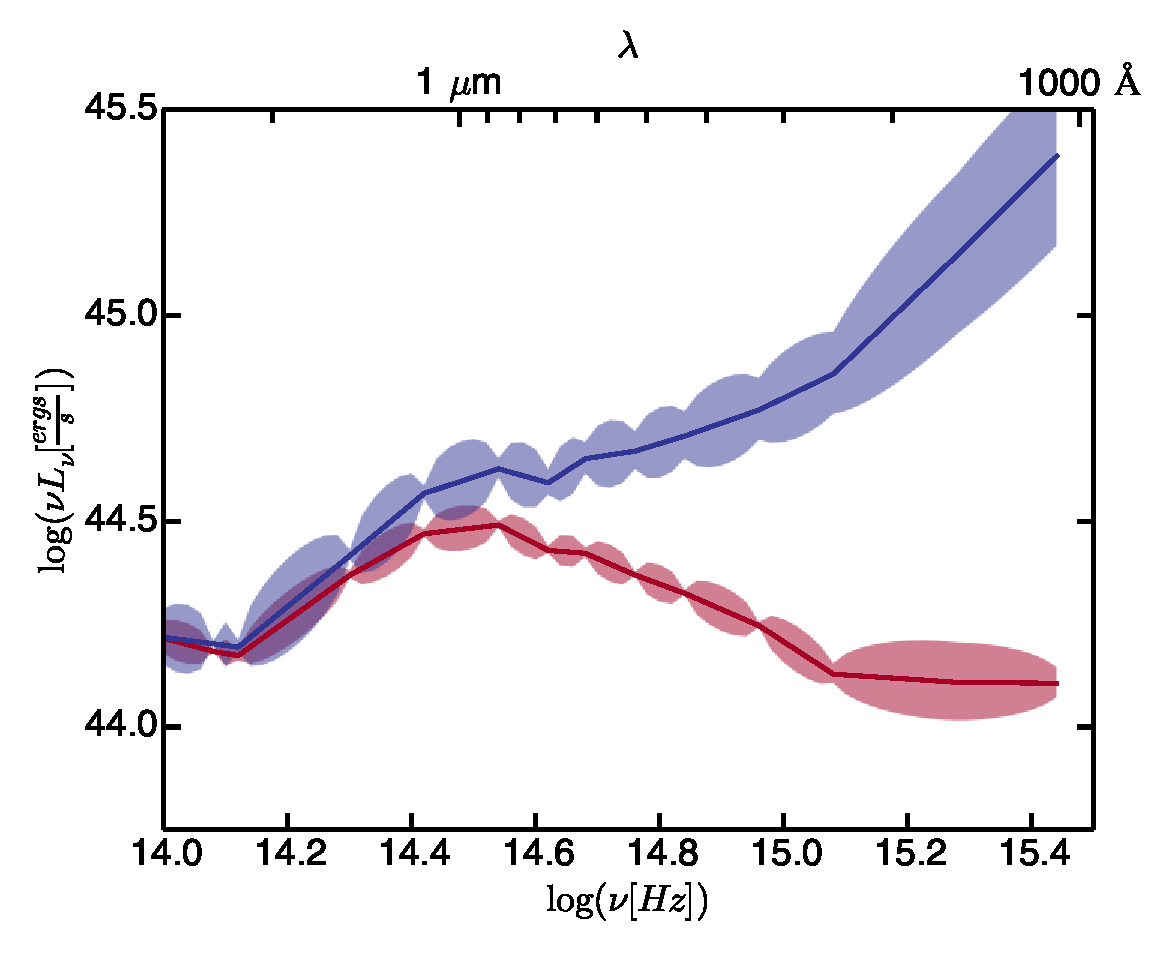
\includegraphics[width=4in]{images/BH/f2}
\caption[Typical reddening correction]{\label{typ_corr} The optical--UV portion of a heavily reddened quasar's SED before (red) and after (blue) correcting for dust reddening.  The (kriged) 1$\sigma$ uncertainty regions are shaded in for both SEDs.  Less than 0.1\% of our sample needs a correction this extreme ($\ebv=0.2$).}
\end{center}
\end{figure}

With the SEDs gap-filled according to their observational properties, we can write Equation~\ref{eqn:red_eq} in terms of the unreddened luminosity and use it to remove the effects of the dust extinction in the SEDs:
%use Equation~\ref{eqn:red_eq} and writing it in terms of the unreddened luminosity we find:
\begin{equation} \label{eqn:sed_dust_remove}
 \log{(\nu L_{\nu{\rm ,\, int}})} = \log{(\nu L_{\nu{\rm ,\, obs}})} + \ebv \frac{R_\lambda}{2.5} 
\end{equation}
where $\nu L_{\nu{\rm ,\, int}}$ is the quasar's intrinsic luminosity, $\nu L_{\nu{\rm ,\, obs}}$ is its observed luminosity, $\ebv$ is the extinction in the ${\rm B-V}$ color, and $R_\lambda$ is a function that is dependent on the type of dust causing the reddening.  To construct SEDs that are free from dust reddening, we began with the individual quasar SEDs from \S\ref{dust_seds}.  Taking the SMC $\ebv$ values from Chapter~\ref{Dust}, we adjust the luminosities to their intrinsic values using Equation~\ref{eqn:sed_dust_remove}. For the uncertainties on $\ebv$ we adopted the mean of the upper and lower $1\sigma$ limits from Table~\ref{tab:ind_fits} and added them in quadrature to the uncertainy in the luminosity for each filter.  This dust correction was applied on top of the corrections from \S\ref{corrections}\footnote{We only apply the correction for dust reddening up to the Ly$\alpha$ line to avoid extrapolating the SMC reddening law into the EUV}.  Figure~\ref{typ_corr} shows an example of a heavily reddened SED before (red) and after (blue) correcting for dust reddening. The SED shown has an $\ebv=0.2$; less than 0.1\% of our sample have corrections this extreme.

To calculate \lbol\, the SEDs need to be extended into the EUV and connected up with the X-ray.  As discussed in detail in \S\ref{EUV}, there are many ways to extend SED into the EUV: connecting the last observed data point to the X-ray with a powerlaw, estimating the 500\,\AA\ point based on luminosity \citep{Scott:2004}, or using a more theoretical model \citep{Casebeer:2006}.  To avoid making additional assumptions about our data, we adopt the first of these methods.  For our luminosity integration range we used \onemum--\twokev.
%For our EUV extension we use the $L$-dependent $\alpha_{\rm FUV}$ relation from \citet{Scott:2004} to connect the observed data to 500\,\AA\ (see \S\ref{EUV} for a more detailed discussion of this method).  This 500\,\AA\ point is connected to 0.2\,keV using the \luvaox\ relation from \citet{Steffen:2006}.  For our luminosity integration range we used \onemum--\twokev.  [expand]
 
\subsection{A Uniform Sample}

\begin{figure}[tp]
\begin{center}
	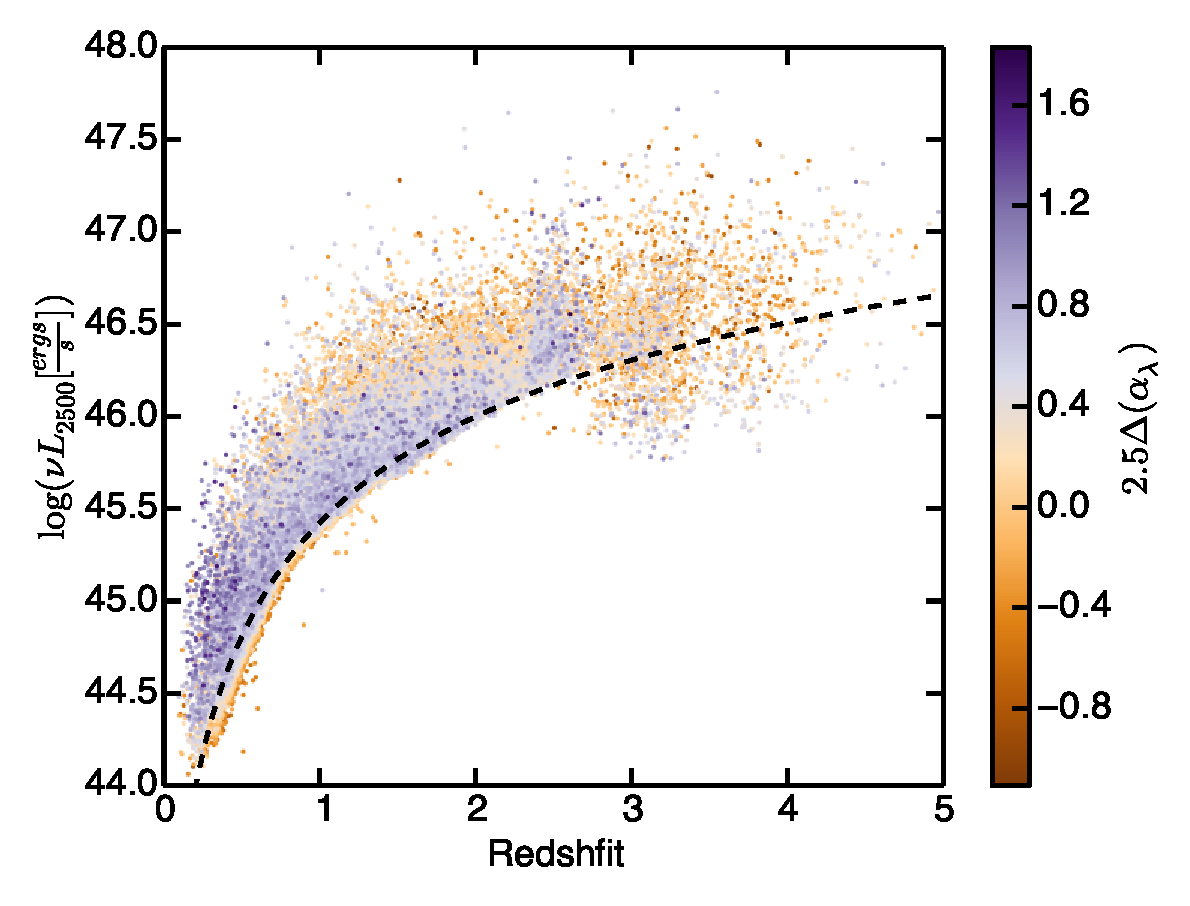
\includegraphics[width=4in]{images/BH/f5}
\caption[Luminosity vs. redshift]{\label{l_z_alpha} \ltwofive\ vs. redshift for our sample of quasars.  The colors indicate the spectral index compared to the mode (see Chapter~\ref{Dust}).  The effects of cutting the sample on $m_i<19.1$ can be clearly seen for $z<2$ in that the redder quasars are seen down to lower intrinsic luminosities than the bluer ones. The black dashed line shows the cut used to remove this bias.}
\end{center}
\end{figure}

As mentioned in \S\ref{Dust_data}, we are only using the uniformly selected quasars from SDSS DR7 \citep{Richards:2006a}.  One of the criteria for this sample is a uniform cut on the {\em observed} $i$-band magnitude of $m_i<19.1$.  Although this works well for creating a uniform sample in the observed-frame, using the \ltwofive\ values for each quasar, we found this sample is not uniform in the rest-frame.  This non-uniformity can be seen in Figure~\ref{l_z_alpha} where we show the (extinction corrected) \ltwofive\ vs. redshift with the color of the data points representing the intrinsic spectral index.  For $z\lesssim2$ we see that the redder quasars are seen down to a lower luminosity than and bluer quasars, a direct artifact of the cut on $m_i$. The reason for this is that at $z\lesssim2$ very blue objects with $m_i=19.1$ necessarily have a larger \ltwofive\ values than red objects with the same $i$-band magnitude, and for $z\gtrsim2$ the trend is reversed ($i$-band$=2500$\,\AA\ at $z\simeq2$).
To create a uniform sample in the rest-frame we define $m_{2500}$ to be the (AB) magnitude associated with \ltwofive:
\begin{equation}
	m_{2500} = 2.5 \times \left[0.738 + 2\log{\left(\frac{D_L}{m}\right)} - \log(1+z) - \log{\left(\frac{\nu L_{\rm 2500\,\AA}}{{\rm erg\, s}^{-1}}\right)}\right]
\end{equation}
where the first term is a constant associated with the AB system, $D_L$ is the luminosity distance, and $z$ is the redshift.  Applying the cut $m_{2500}<19.1$ (black dashed line in Figure~\ref{l_z_alpha}) removes the bias caused by the cut on the $i$-band magnitude.  If this cut was not made our analysis would be able to properly marginalize over luminosity trends in the SEDs since the low redshift red quasars extend to lower luminosities than the low redshift blue quasars.

%\subsection{\ltwofive\ and \bctwofive\ Distributions} \label{l_bc_dust}
\subsection{Extinction Corrected SEDs} \label{l_bc_dust}
\begin{figure}[t]
\begin{center}
\begin{tabular}{cc}
	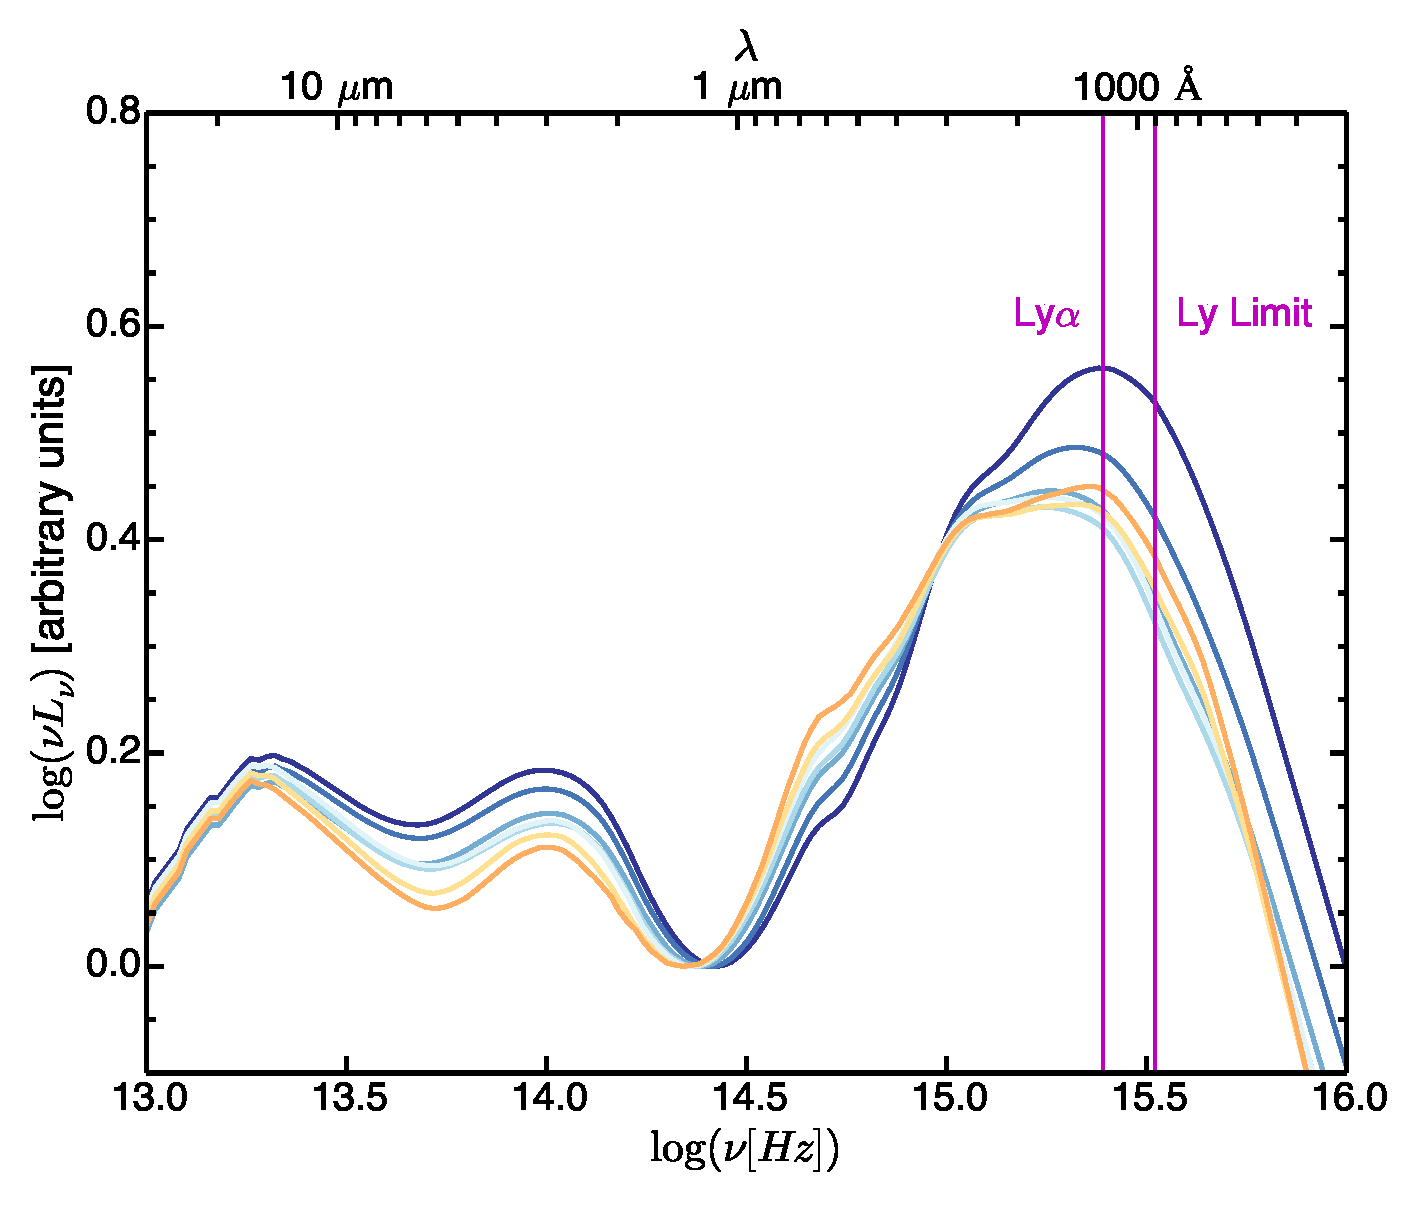
\includegraphics[width=3in]{images/BH/f4a} & 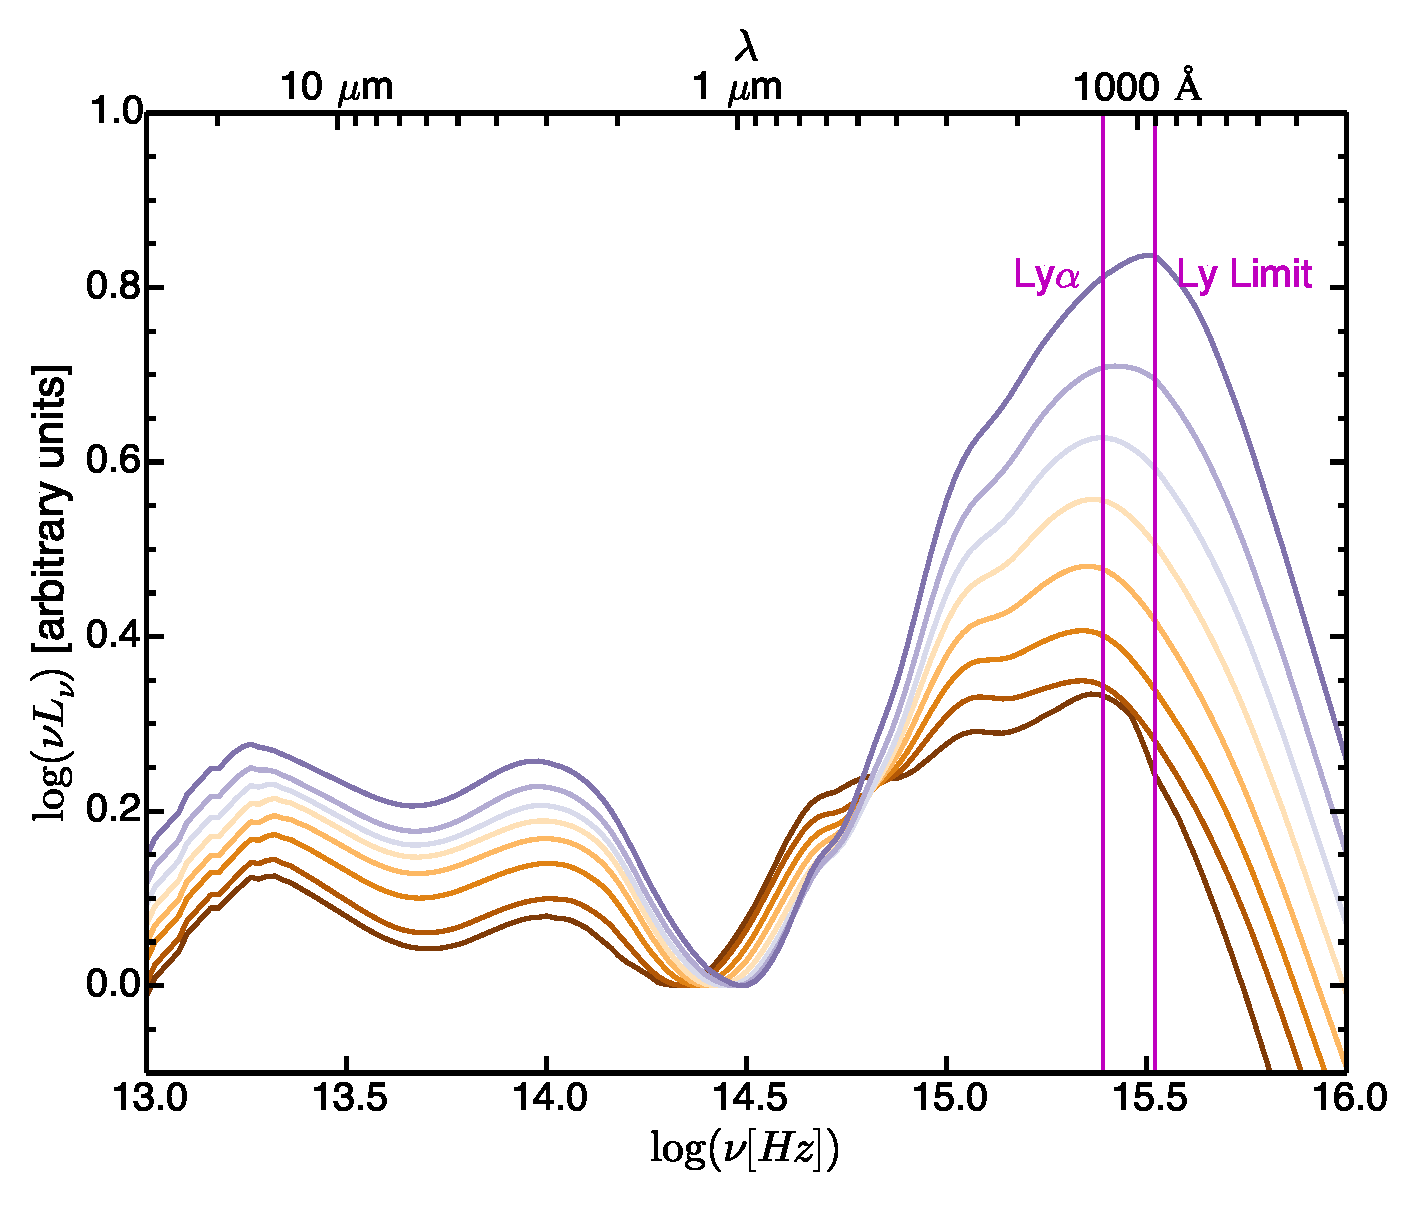
\includegraphics[width=3in]{images/BH/f4b} \\
	\hspace{.5cm} 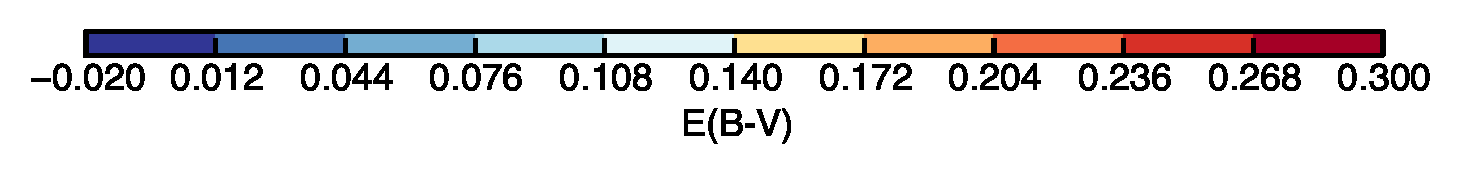
\includegraphics[width=2.75in]{images/BH/ebv_colorbar} & \hspace{.5cm} 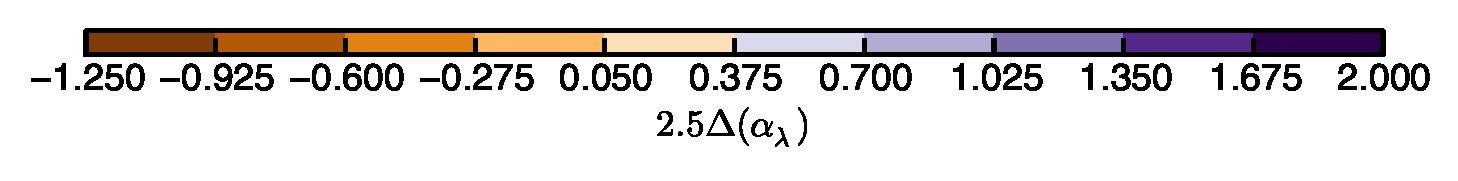
\includegraphics[width=2.75in]{images/BH/alpha_colorbar}
\end{tabular}
\caption[Mean corrected SEDs grouped by dust and color]{\label{sed_dust_color_rc} Redshift matched and extinction corrected SEDs as a function of $\ebv$ ({\em left}) and intrinsic color ({\em right}).  {\em Left}: SEDs with more dust extinction show less hot dust and a redder spectral index between 5--11\,$\mu$m. {\em Right}: Intrinsically bluer quasars show more hot dust emission and have their BBBs peak at shorter wavelengths than the red quasars.  The bluest mean SED has $\alpha_\nu \sim 0.03$.  All SEDs have been normalized at their minimum value near \onemum.}
\end{center}
\end{figure}

With this newly-defined uniform sample and extinction corrected SEDs we are able to explore the mean SEDs as functions of color and extinction.  Figure~\ref{sed_dust_color_rc}  shows the mean SEDs based on $\ebv$ ({\em left}) and intrinsic color ({\em right}) after marginalizing over the other variables (e.g. the blue line in the left panel shows the mean SED for all quasars with $\ebv<0.012$ regardless of intrinsic color).  To ensure the differences seen in the mean SEDs are being caused by the variable of interest, the redshift distribution for each SED have been matched within each panel.  When making the uniform redshift distributions we dropped the three bins with the most dust extinction and the two intrinsically bluest bins due to low number counts ($< 100$ quasars in the bin).

\begin{figure}[t]
\begin{center}
\begin{tabular}{c}
	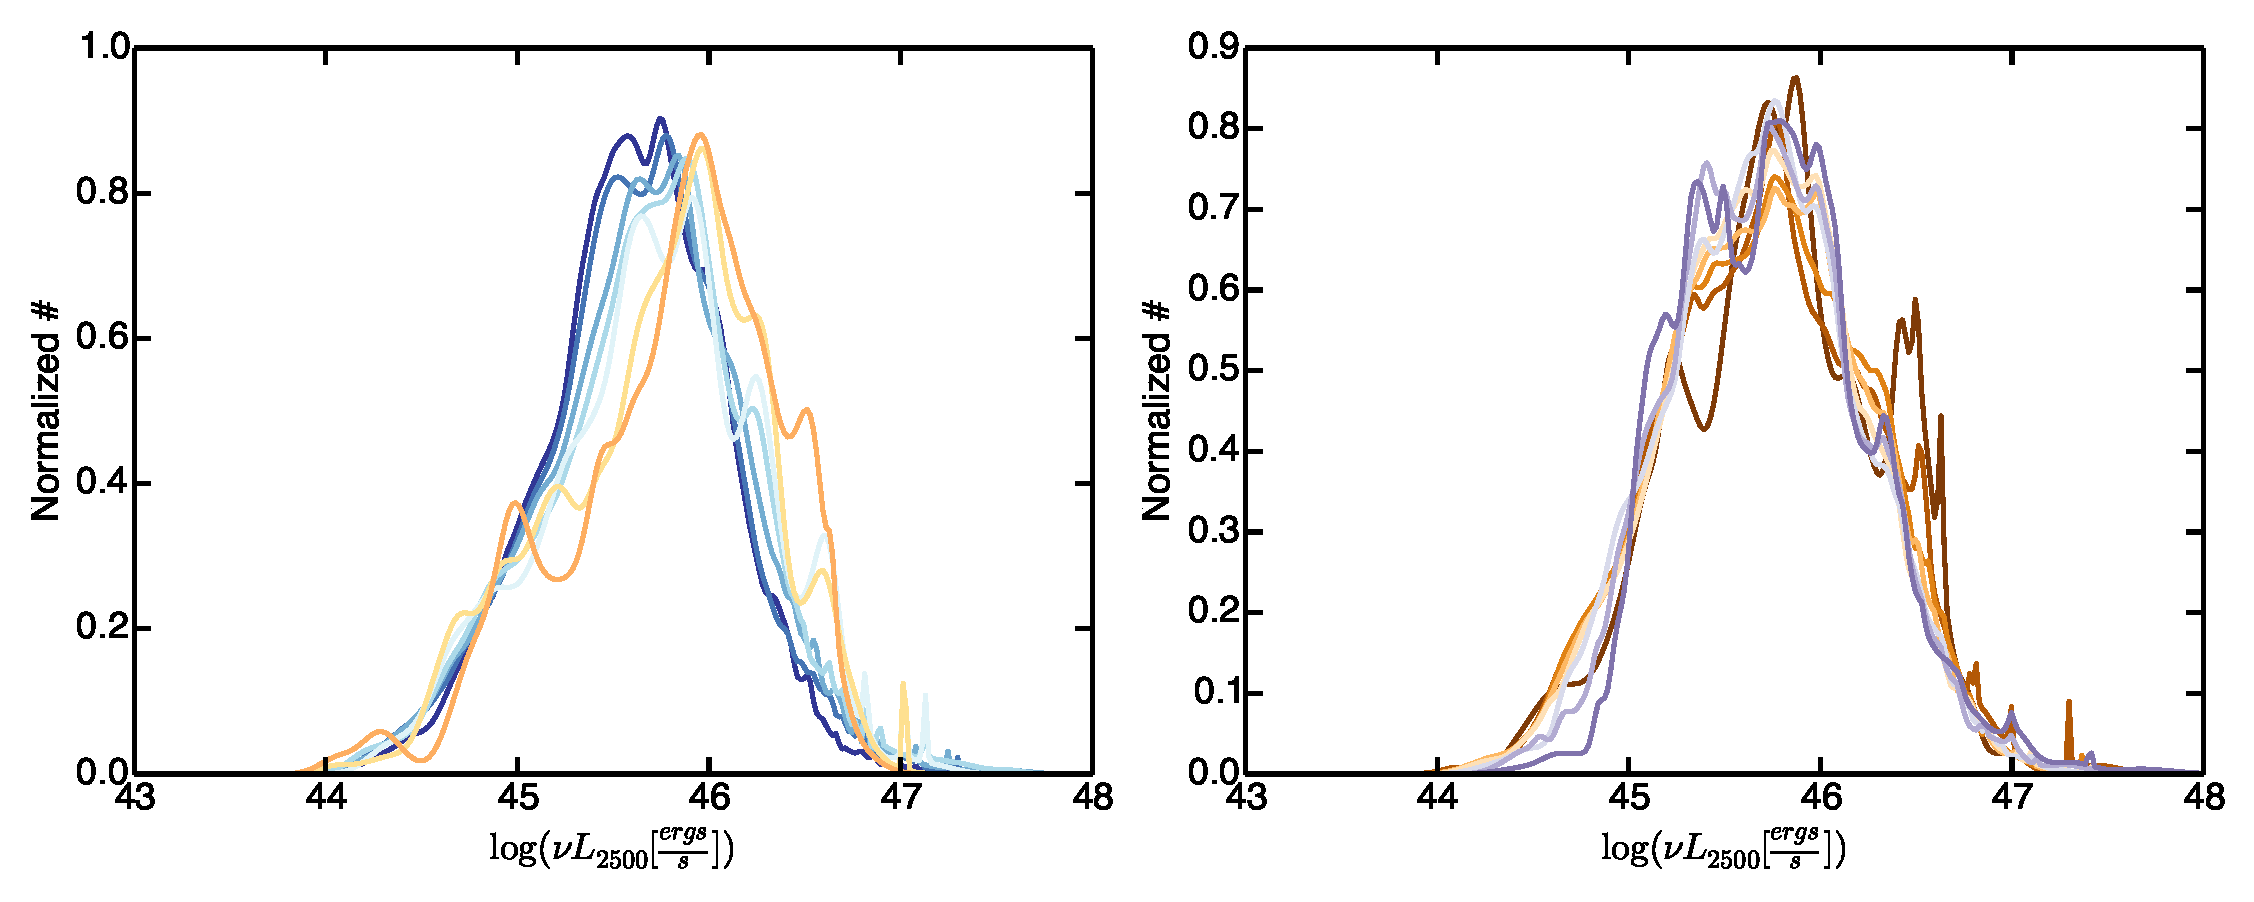
\includegraphics[width=5.5in]{images/BH/f6a} \\
	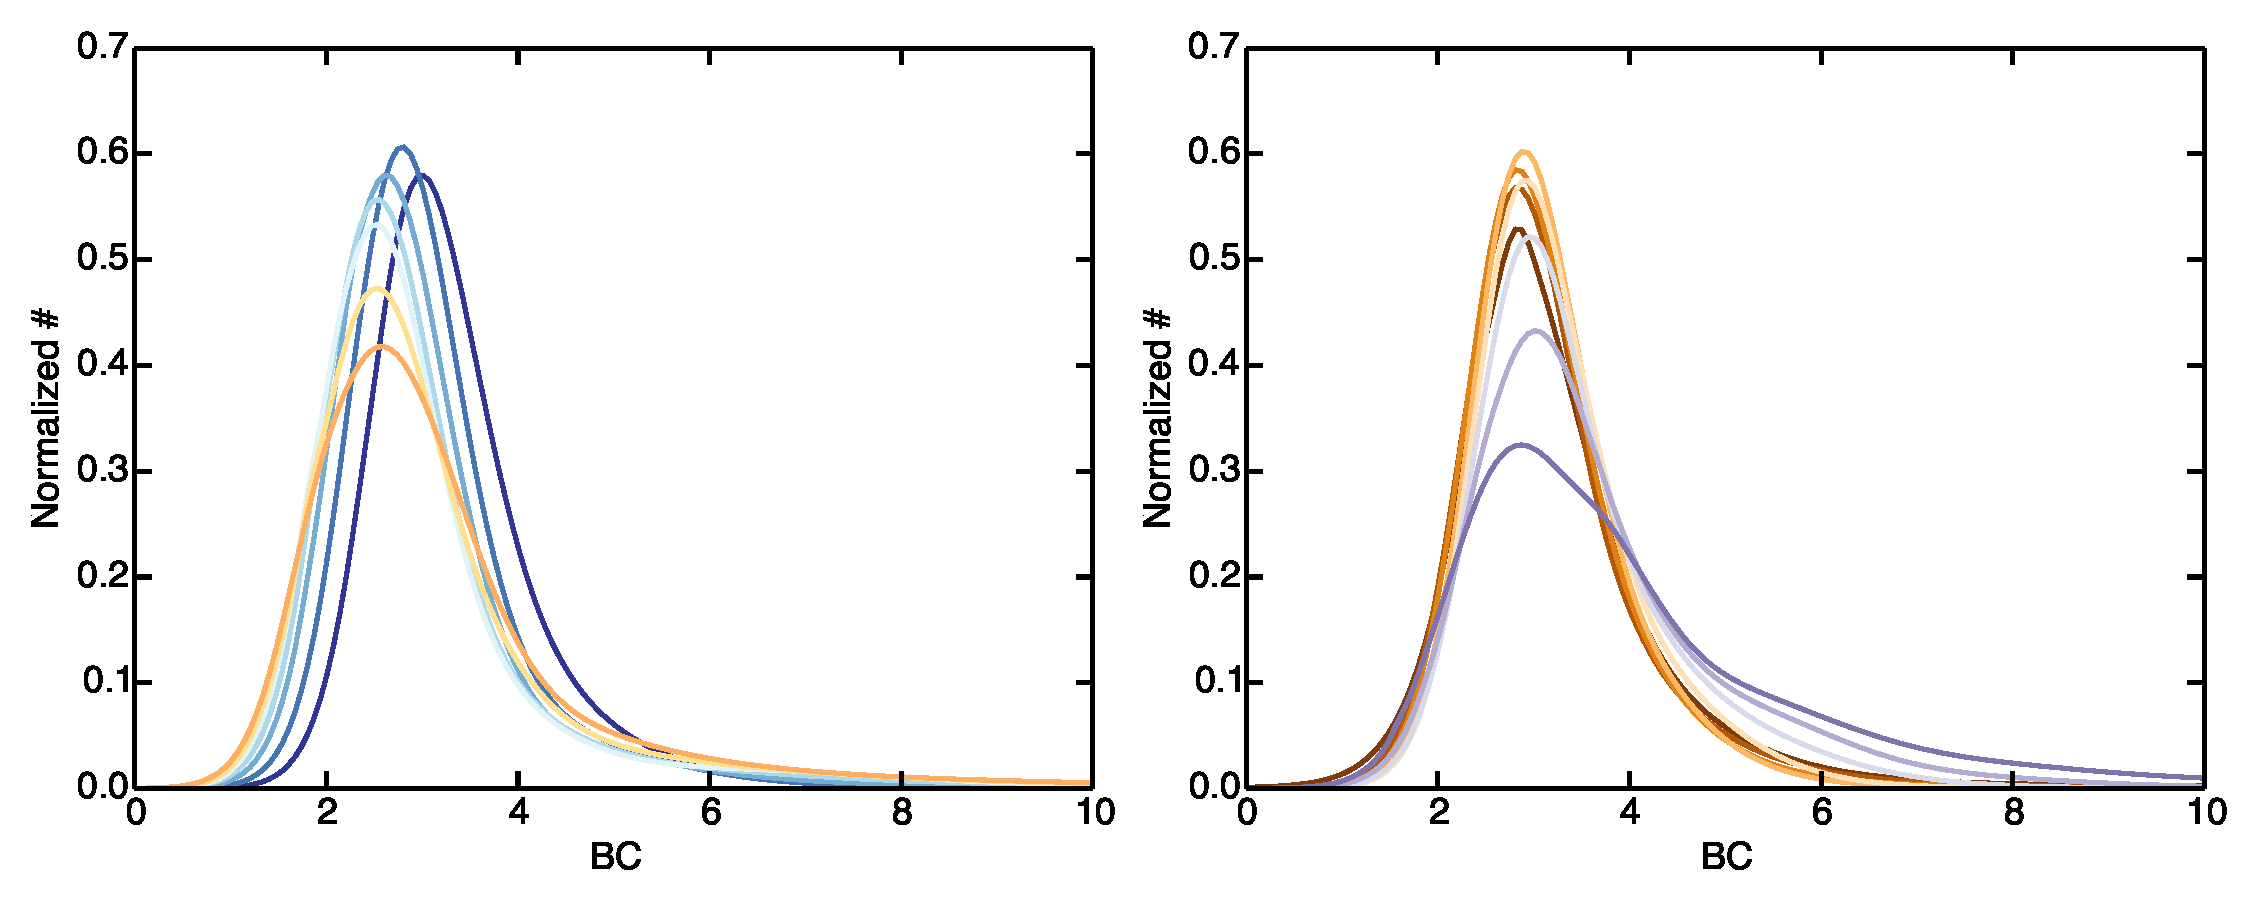
\includegraphics[width=5.5in]{images/BH/f6b} 
\end{tabular}
\begin{tabular}{cc}
	\hspace{.4cm} 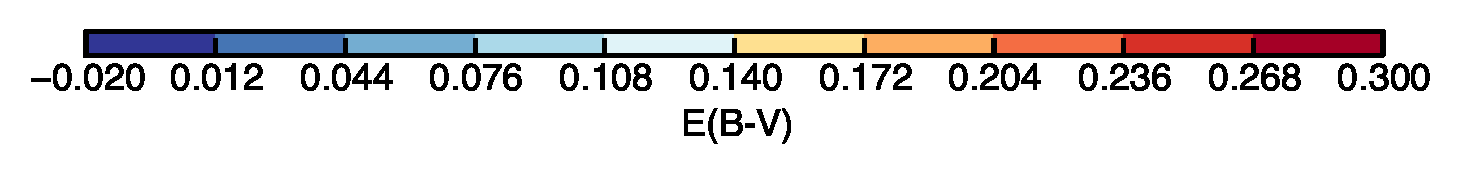
\includegraphics[width=2.5in]{images/BH/ebv_colorbar} & \hspace{.4cm} 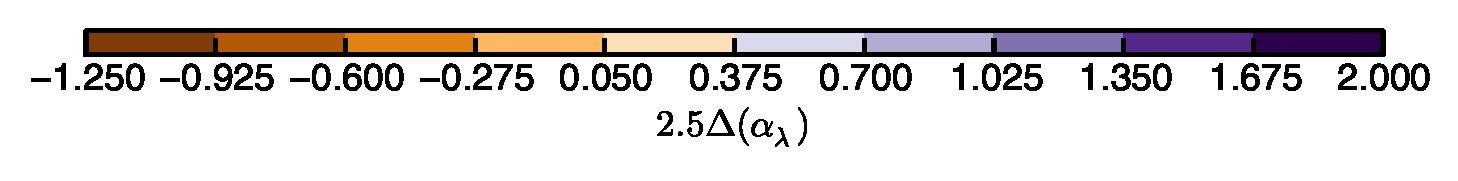
\includegraphics[width=2.5in]{images/BH/alpha_colorbar}
\end{tabular}
\caption[\ltwofive\ and \bctwofive\ distributions grouped by dust and color]{\label{L_BC_dust_color_rc} The fully marginalized \ltwofive\ ({\em top}) and \bctwofive\ ({\em bottom}) distributions for $\ebv$ bins ({\em left}) and for intrinsic color bins ({\em right}).  From the \ltwofive\ plots we can see that the dusty quasars are intrinsically more luminous while there are no trends in luminosity with intrinsic color.
The \bctwofive\ plots show a trend for more reddened quasars have smaller \bctwofive, while intrinsic color shows bluer quasars have larger \bctwofive.
%, perhaps an indication of an inclination effect. There is also a trend in intrinsic color where bluer quasars to have larger \bctwofive.
}
\end{center}
\end{figure}

With the fully stacked SEDs, the trend in $\ebv$ seen in the mid-IR from Figure~\ref{sed_dust} has become stronger (left panel of Figure~\ref{sed_dust_color_rc}).  The spectral index from 5--11\,$\mu$m becomes redder as the amount of dust extinction increases. The differences in these SEDs indicate there is a sample selection and/or intrinsic effect that is a function of $\ebv$.  If this were not the case, all differences in the SEDs would be averaged away.  A full analysis of the possible causes for these differences is beyond the scope of this work.
%This trend shows that although the quasars with more dust extinction have less hot dust, they do have more total dust.

As in Figure~\ref{sed_color}, we find bluer quasars have more hot dust emission than redder quasars (right panel of Figure~\ref{sed_dust_color_rc}). Additionally, their big blue bumps (BBBs) also peak at shorter wavelengths, consistent with the bluer quasars having a hotter accretion disk.  However, this seems to be in contention with the stacked spectra from \S\ref{sec:spectra} where the bluer quasars had weaker ionized spectral lines, indicating they have less ionizing radiation in the range of $\sim$200--1000\,\AA ($\sim$12--60\,eV).  If the bluer quasars have their BBB peak at shorter wavelengths we would naively expect them to also have more ionizing radiation, and stronger ionized spectral lines. One explanation for this discrepancy is if the redder quasars have an extra SED component in the unseen EUV at $\sim$50eV \citep[e.g.,][]{Done:2012}.

Another possible explanation for this discrepancy is inclination angle. As the inclination angle is increased from face-on to edge-on, the apparent SED becomes bluer, \ltwofive\ becomes smaller, and the BBB is shifted to shorter wavelengths \citep[see Figure~2 from][]{Sun:1989}.  These changes are correlated such that \lbol\ is independent of inclination, resulting is an increase in \bctwofive.  Although the observed SED has more ionizing radiation, the broad line region (BLR) is seeing the accretion disk closer to face-on, and as a result, sees {\em less} ionizing radiation.  This idea that the BLR sees a different continuum than we do is not a new one; \citet{Korista:1997} was lead to the same conclusion when trying the reconcile the emission lines of Mrk 335 with the observed EUV continuum.
However, not all of the changes in the intrinsic color SEDs can be attributed to inclination, since the \ltwofive\ distribution is the same for all of the color bins (see Figure~\ref{L_BC_dust_color_rc}).

Using these SEDs we also look at the distributions for \ltwofive\ and \bctwofive\ as functions of intrinsic color and $\ebv$.  This was done by modeling the probability distribution for the parameter of interest (e.g. \ltwofive\ or \bctwofive) as a normal distribution centered on the measured value and having a width given by the 1$\sigma$ uncertainty.  This distribution is weighted by the likelihood that the quasar belongs to a given color or $\ebv$ bin and all distributions belonging to a common bin are summed together and the result is normalized such that it integrates to unity.

Figure~\ref{L_BC_dust_color_rc} show the resulting marginalized distributions for \ltwofive\ ({\em top}) and \bctwofive\ ({\em bottom}) for $\ebv$ bins ({\em left}) and intrinsic color bins ({\em right}).  For \ltwofive\ we only see a tend with $\ebv$.  There are (relatively) more high luminosity quasars with high dust extinction than low dust extinction.

%see trends in both samples. There are (relatively) more low luminosity quasars in the more heavily reddened and bluer quasars. It is interesting to note that even though the SEDs for the bluer quasars look the most similar to the high-luminosity SED from \S\ref{Luminosity SED} it actually contains the most low luminosity quasars. However,  we can't make a direct comparison between these SEDs and the SEDs from \S\ref{Luminosity SED} since the quasars used to make the luminosity-dependent SEDs have a narrow redshift distribution, and the SEDs constructed here don't have the same constraint.

\begin{figure}[t]
\begin{center}
\begin{tabular}{cc}
	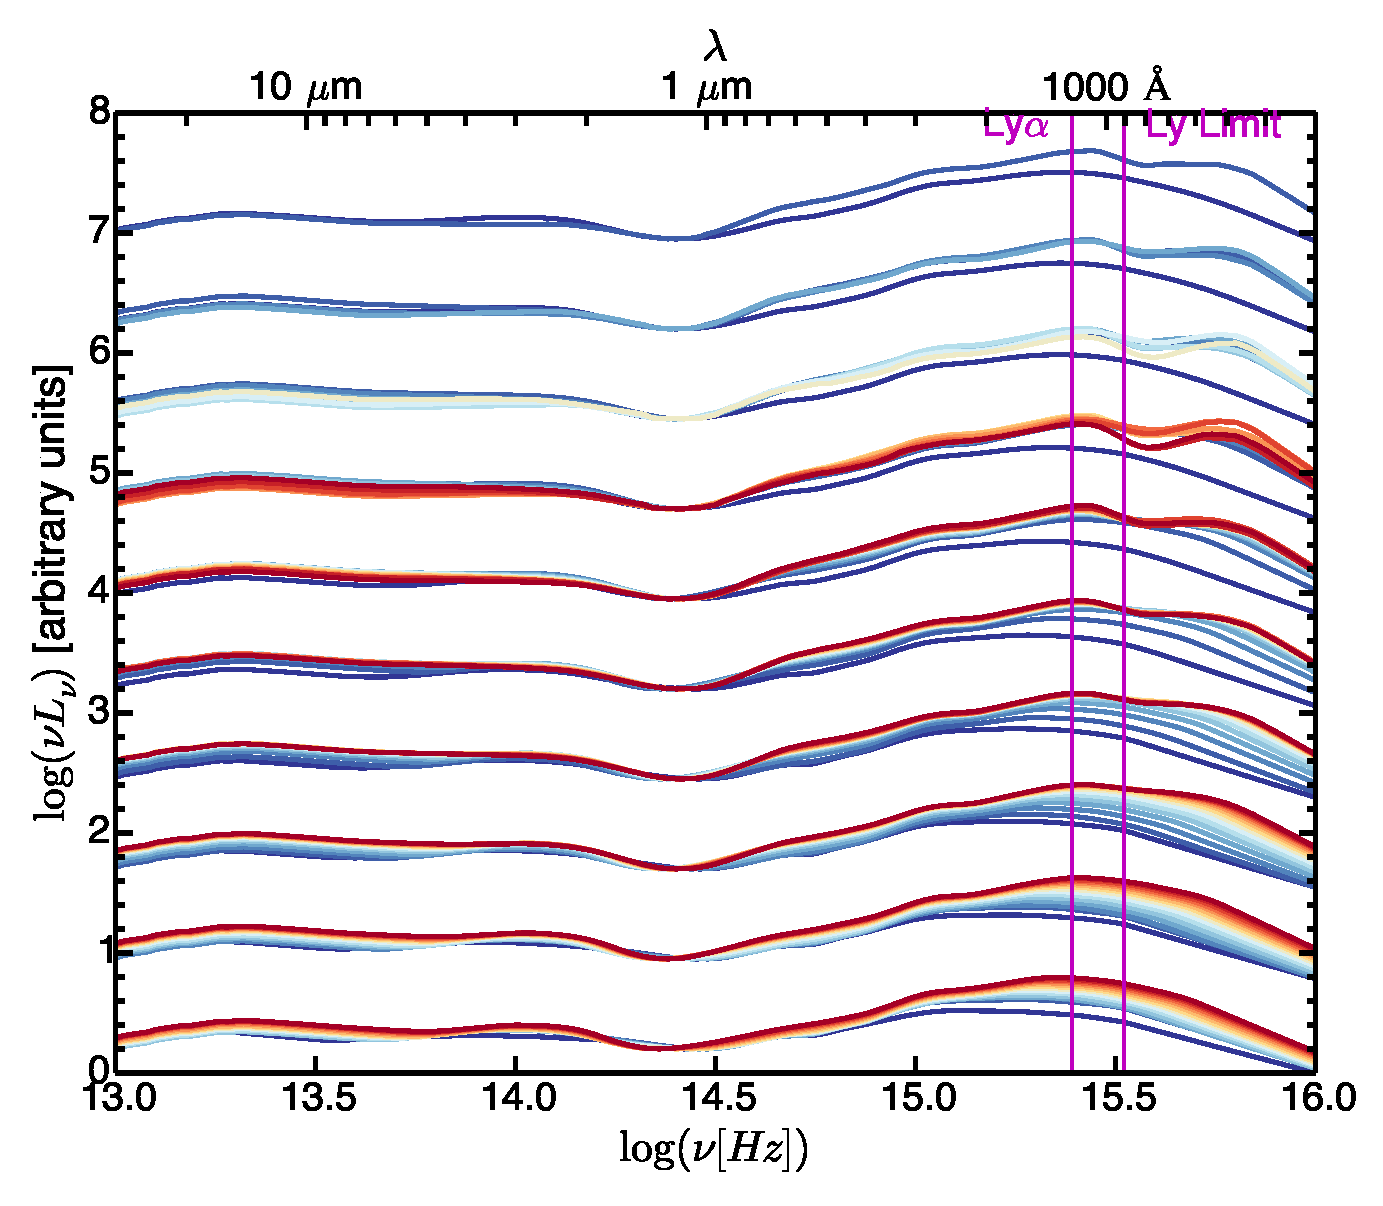
\includegraphics[width=4in]{images/BH/f7a} & 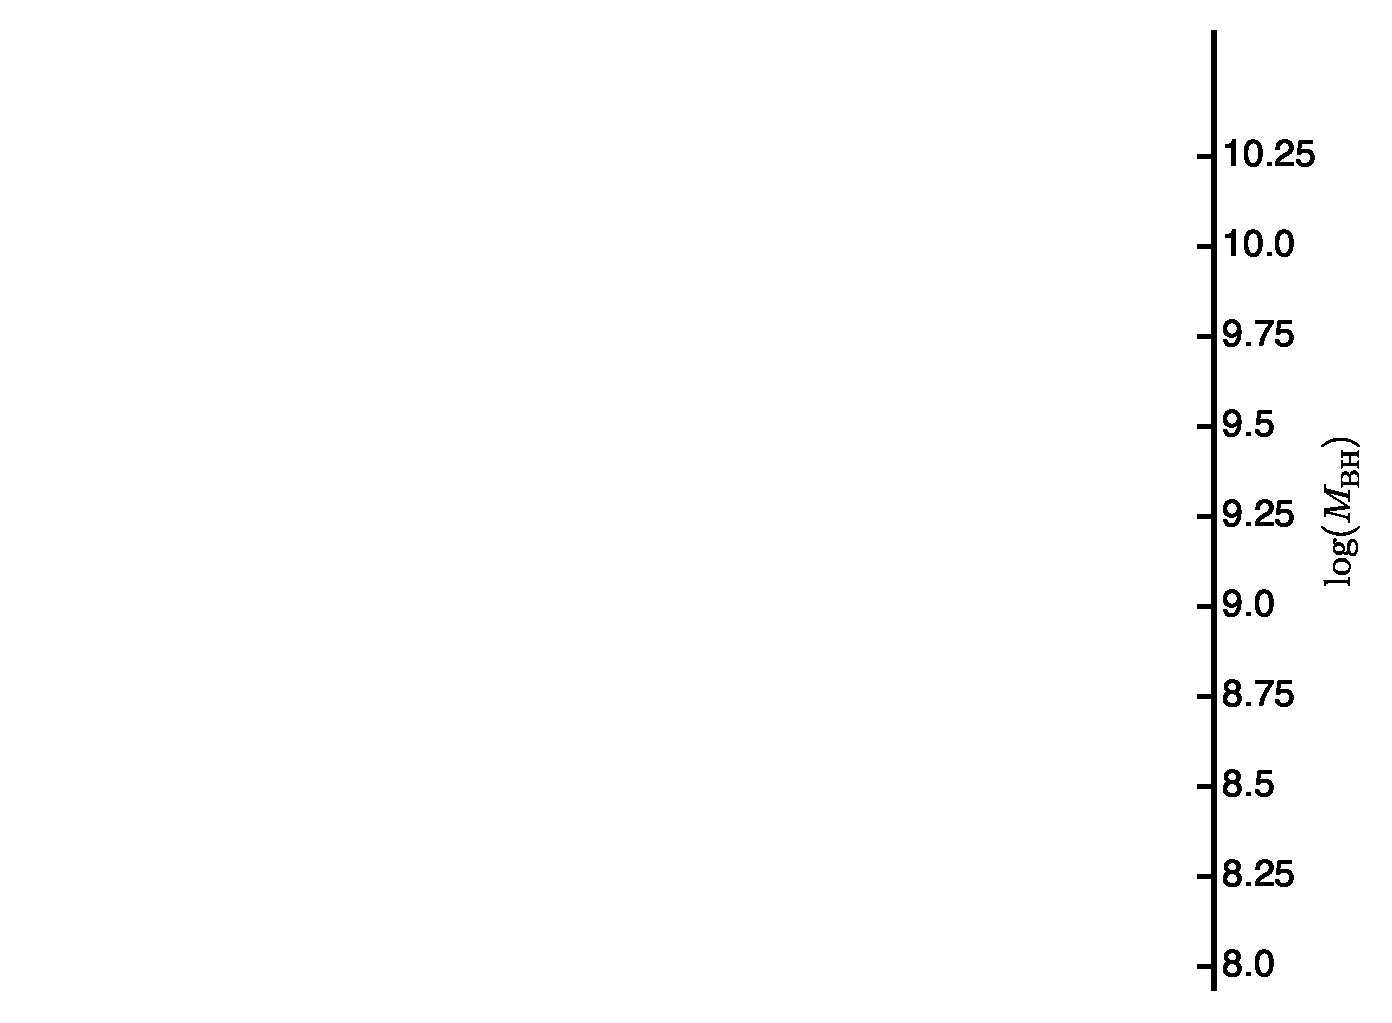
\includegraphics[trim={7.8in -.65in 0 0}, clip=true, height=3.25in]{images/BH/M_ticks}\\
	\hspace{.4cm} 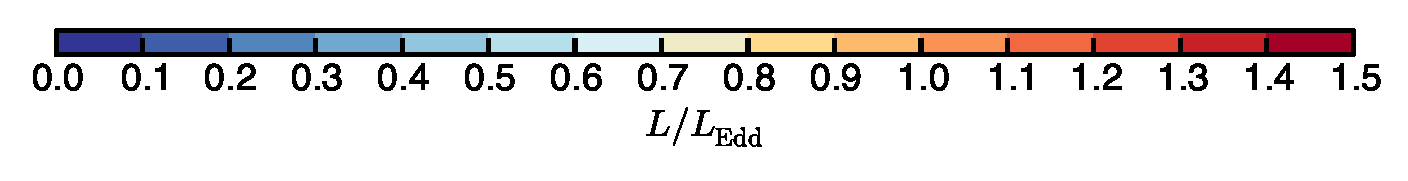
\includegraphics[width=3.75in]{images/BH/Lf_colorbar} &
\end{tabular}
\caption[Mean SEDs grouped by $\mbh$]{\label{Lfrac_sed} Mean SEDs for quasars grouped by $\mbh$ with the most massive SEDs on the top and the colors indicating $\lf$. As $\lf$ increases the peak of the BBB shifts to lower wavelengths, indicating a hotter accretion disk.  All SEDs have been normalized at their minimum near \onemum\ and each grouping has been offset vertically for clarity.}
\end{center}
\end{figure}

\begin{figure}[t]
\begin{center}
\begin{tabular}{cc}
	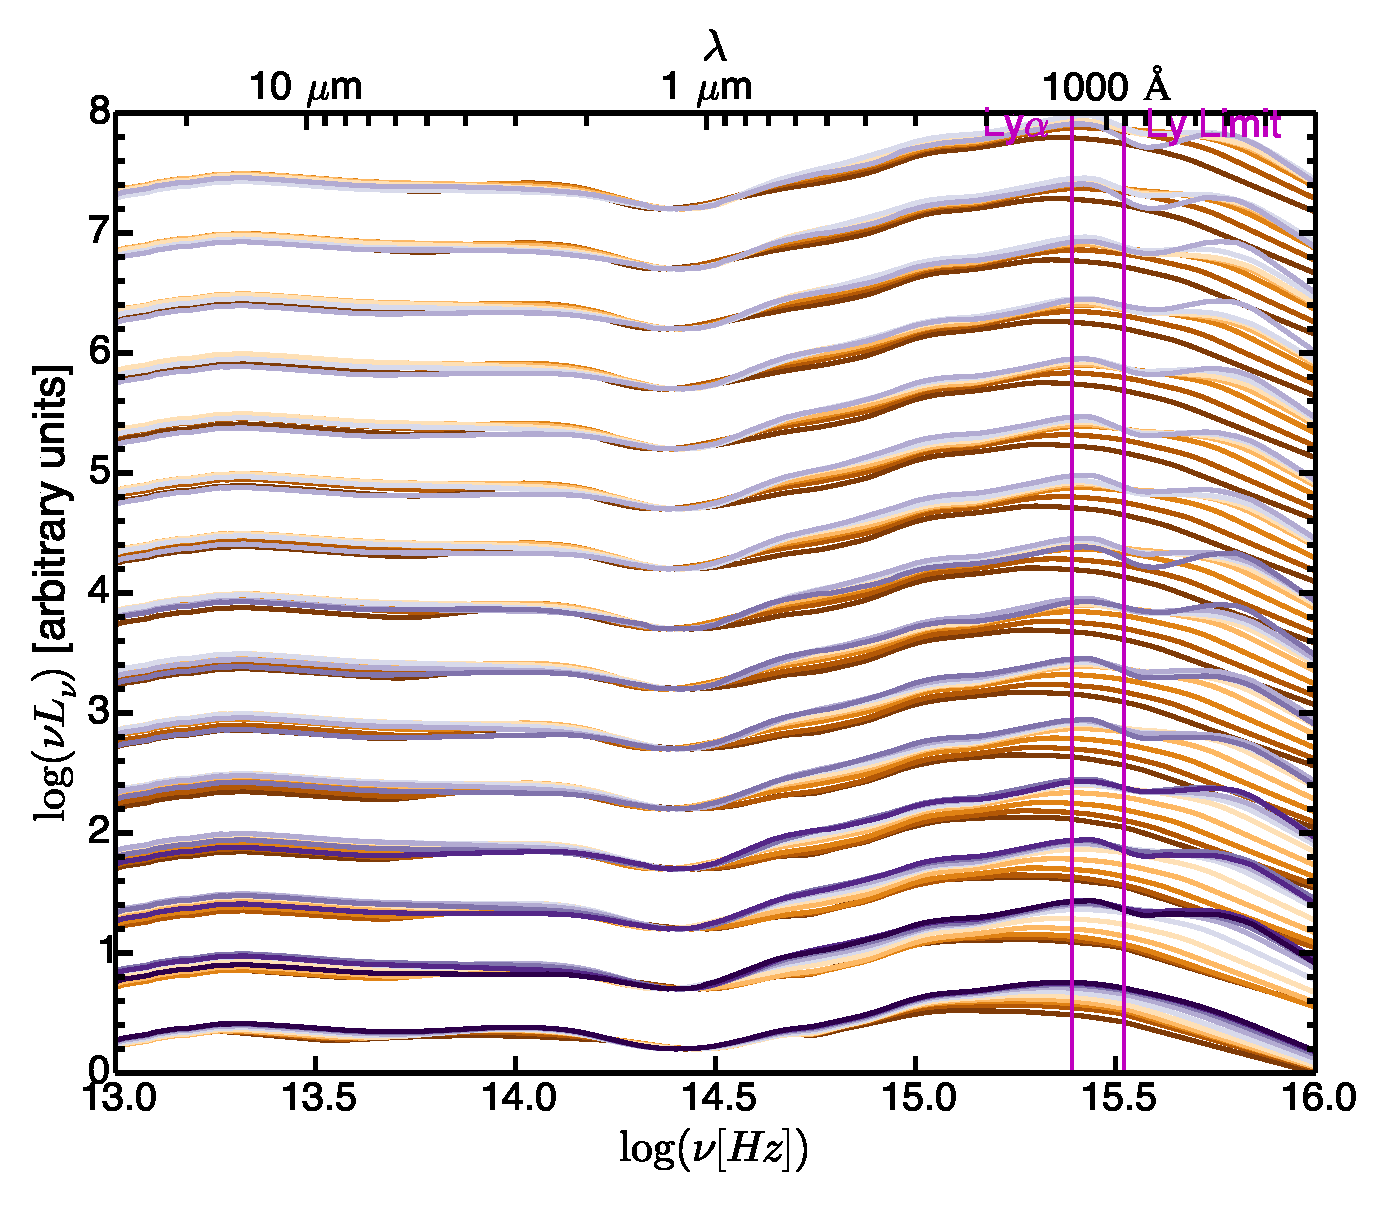
\includegraphics[width=4in]{images/BH/f7b} & 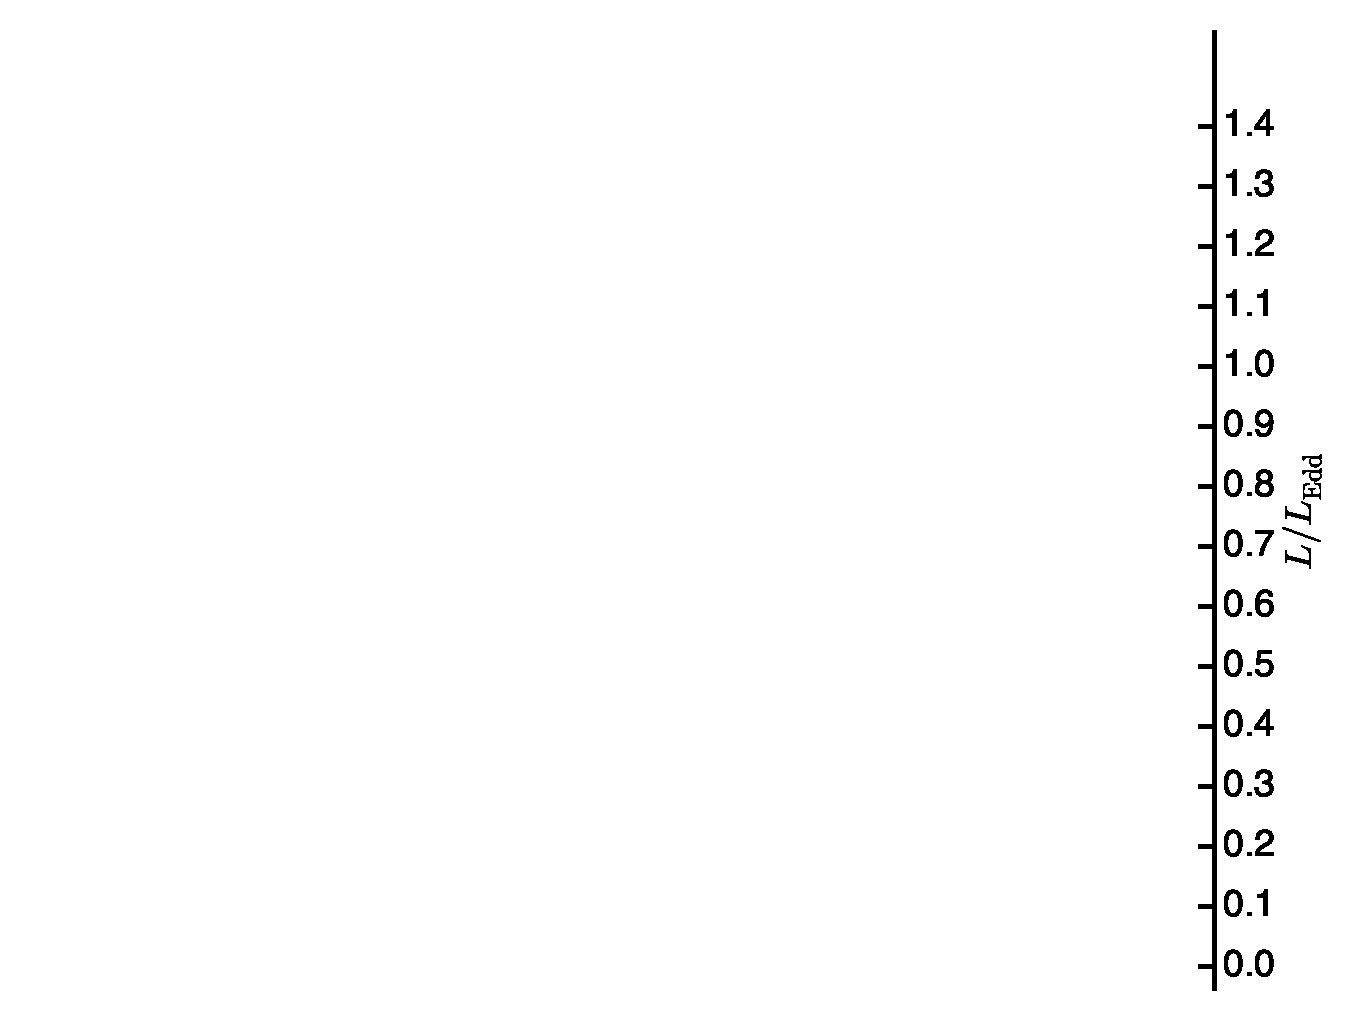
\includegraphics[trim={7.8in -.65in 0 0}, clip=true, height=3.25in]{images/BH/L_ticks}\\
	\hspace{.4cm} 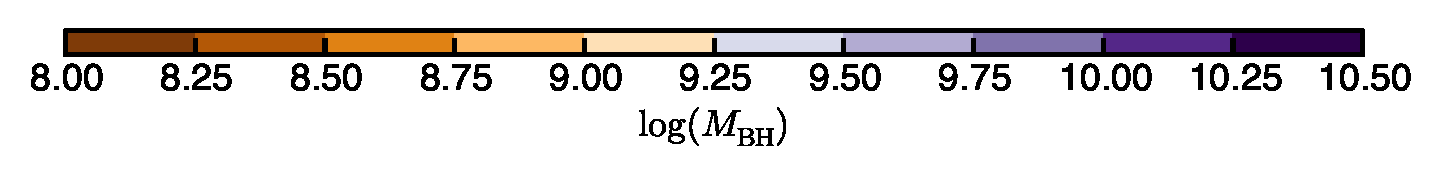
\includegraphics[width=3.75in]{images/BH/M_colorbar} &
\end{tabular}
\caption[Mean SEDs grouped by $\lf$]{\label{Mbh_sed} Mean SEDs for quasars grouped by $\lf$ with the largest ratio on the top and the colors indicating $\mbh$. The higher mass SEDs show an initial peak in the BBB at shorter wavelengths than the low mass SEDs and also show an extra bump in the EUV (see text).  All SEDs have been normalized at their minimum near \onemum\ and each grouping has been offset vertically for clarity.}
\end{center}
\end{figure}

For both parameters we see trends in the {\em corrected} \bctwofive\ distributions.  In the lower left panel of Figure~\ref{L_BC_dust_color_rc} we see \bctwofive\ becomes smaller as $\ebv$ increases, a result of their higher \ltwofive\ distribution. Looking at the trends with intrinsic color we see the bluer quasars have (on average) higher \bctwofive.  As stated earlier, this trend could be caused by inclination effects, where some of the bluer quasars are viewed closer to edge-on.

%This correlation could be caused by an inclination effect: quasars viewed more edge-on appear less luminous [find ref for this], causing smaller \bctwofive, and our line of sight to the quasar passes through more of the dusty torus around the accretion disk, causing higher extinction.  Looking at \bctwofive\ as a function of intrinsic color there is a clear trend where bluer quasars have higher \bctwofive.  [cmk: The more I think about this the more backwards it seems... edge-on SEDs have lower \ltwofive\ and \lbol\ is independent of inclination. You would expect edge-on disks to have larger BC, not smaller.  The trends we see would be consistent with high $\ebv$ indicating a face-on disk.]
%For the two bluest bins the distribution becomes bimodal.  Taking a closer look at these quasars we found this was caused by the bluer quasars not having uniform coverage in redshift space.  The bluer quasars are concentrated in two groups: low redshift ($z<1$) with low luminosity, and high redshift ($z>2.5$) with high luminosity (see Figure~\ref{l_z_alpha}).  This split gives rise to bimodal distribution seen in \bctwofive.

\section{SEDs Based on $\mbh$ and $\lf$} \label{mbh_seds}

The standard optically-thick geometrically-thin accretion disk from \citet[][see \S\ref{sec:AD} for a review of the $\alpha$-disk model]{Shakura:1973} predicts that the temperature of the disk is proportional to the accretion rate ($\dot{M}/\dot{M}_{\rm Edd}$) and inversely proportional to $\mbh$ (see Equation~\ref{disk_temp}). If a quasar's spectral index is heavily influenced by the turnover in the BBB, the $\alpha$-disk model would predict quasars with higher accretion rates to be bluer and quasars with higher $\mbh$ to be redder.  We can test this prediction by constructing SEDs based on our estimated values of $\mbh$ (\S\ref{BH_data}) and using the Eddington fraction:
\begin{equation} \label{lf_eqn}
	%\lf = \frac{L_{\rm bol}}{L_{\rm Edd}} = \frac{\dot{M}}{\dot{M}_{\rm Edd}}
	\frac{\dot{M}}{\dot{M}_{\rm Edd}} = \frac{L}{L_{\rm Edd}} = \frac{L_{\rm bol}}{L_{\rm Edd}} \propto \frac{L_{\rm bol}}{M_{\rm BH}}
\end{equation}
as a proxy for the accretion rate (see \S\ref{Eddington_fraction}). From the final proportionality we can see that the accretion rate is also inversely proportional to $\mbh$, so to isolate changes in the quasar's SEDs that are only caused by changes $\mbh$ or $\lf$ it is important to hold the other variable in a fixed range.  
%This is done by splitting our sample into bin in $\mbh$--$\lf$ parameters space.

As we did for the quasars' color and dust properties in \S\ref{dust_seds}, we bin our data based on the measured values for $\lmbh$ and $\lf$.  Since these parameters are correlated  (see Equation~\ref{lf_eqn}) and not known to high accuracy, we weight each quasar by its probability of belonging to each bin.
To find these weights we use a Monte Carlo (MC) method: for each quasar we simulate 10,000 $\lmbh$ and $\log{(L_{\rm bol})}$ values taken from (uncorrelated) normal distributions centered on the measured values and having widths equal to the $1\sigma$ uncertainties. Each pair of simulated values were used to calculate a simulated $\lf$, keeping intact the covariance between $\lf$ and $\lmbh$.  The fraction of simulated points landing in each bin gives an estimate for the probability of the quasars belonging to that bin.
%The simulated values for $\lmbh$ and $\lf$ were used to find the probability that the quasar belongs to each of the bins in $\lmbh$--$\lf$ space.

\begin{figure}[t]
\begin{center}
\begin{tabular}{c}
	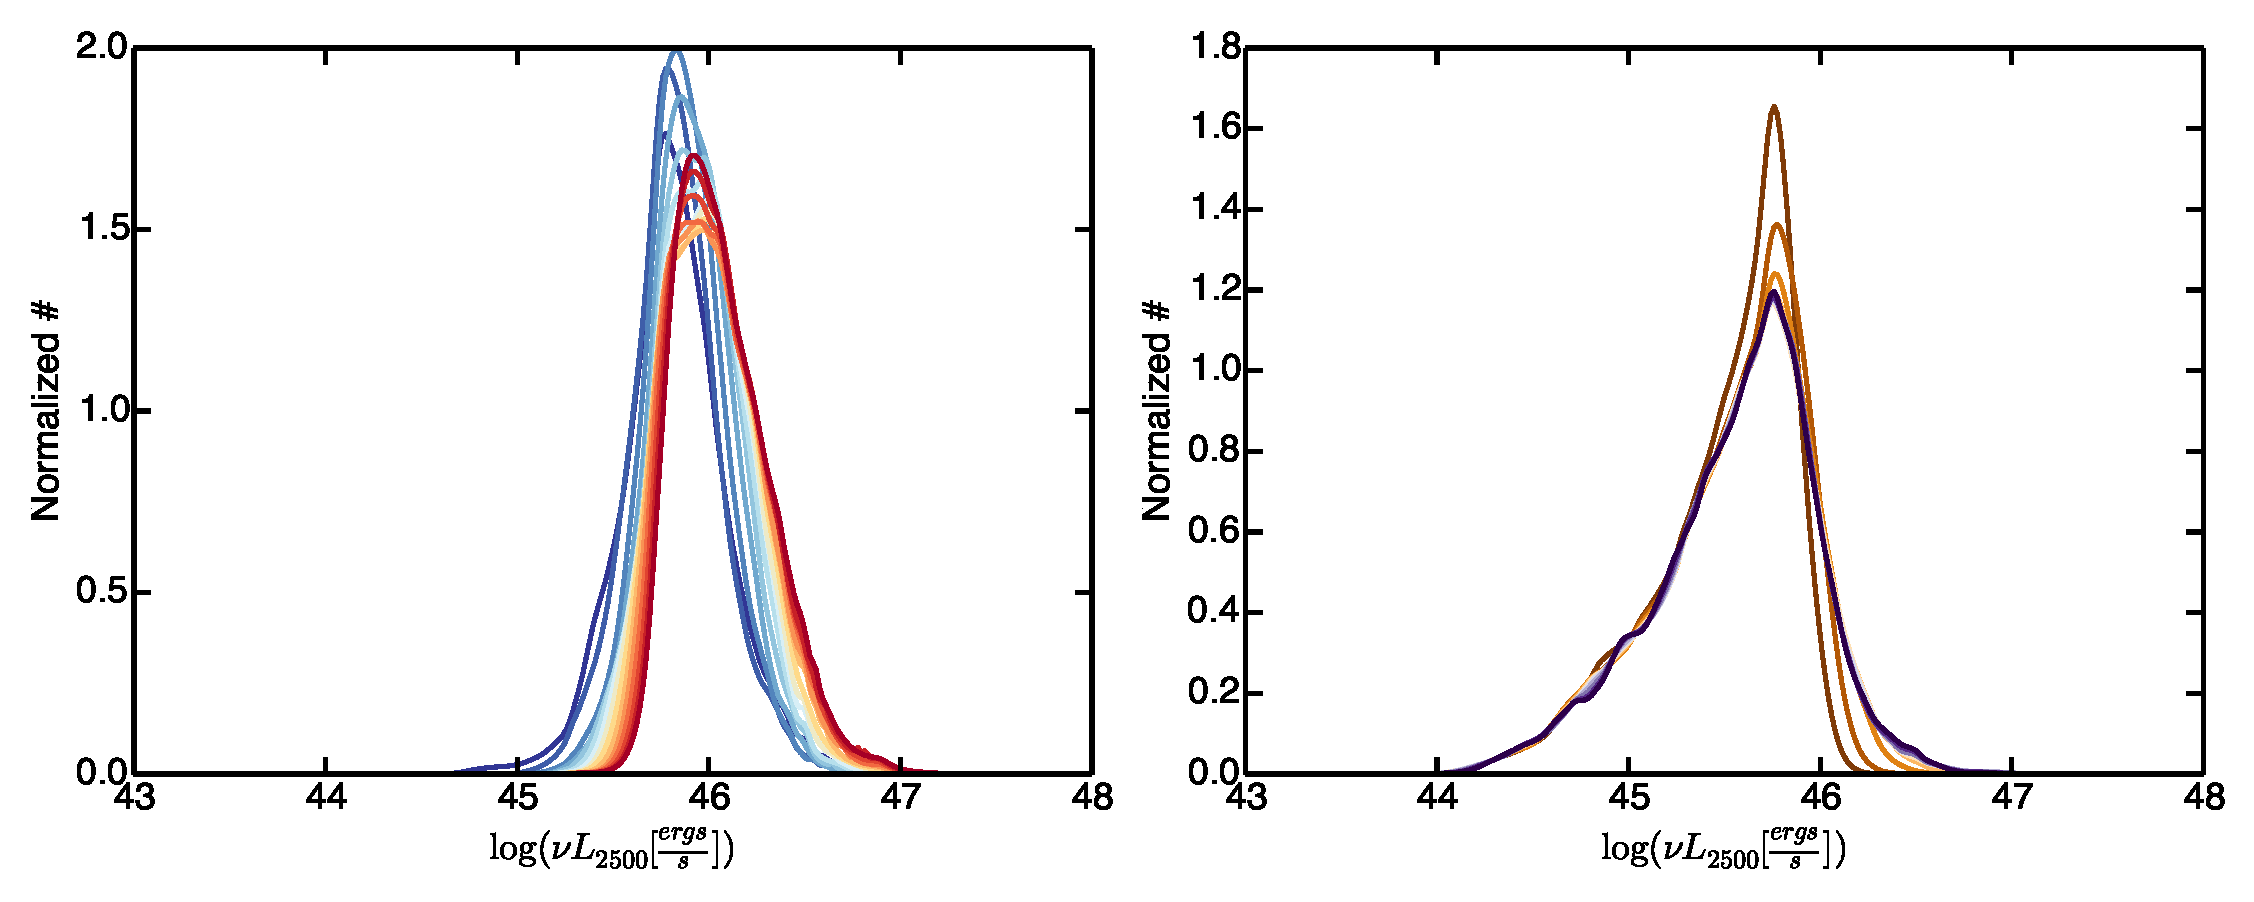
\includegraphics[width=5.5in]{images/BH/f8a} \\
	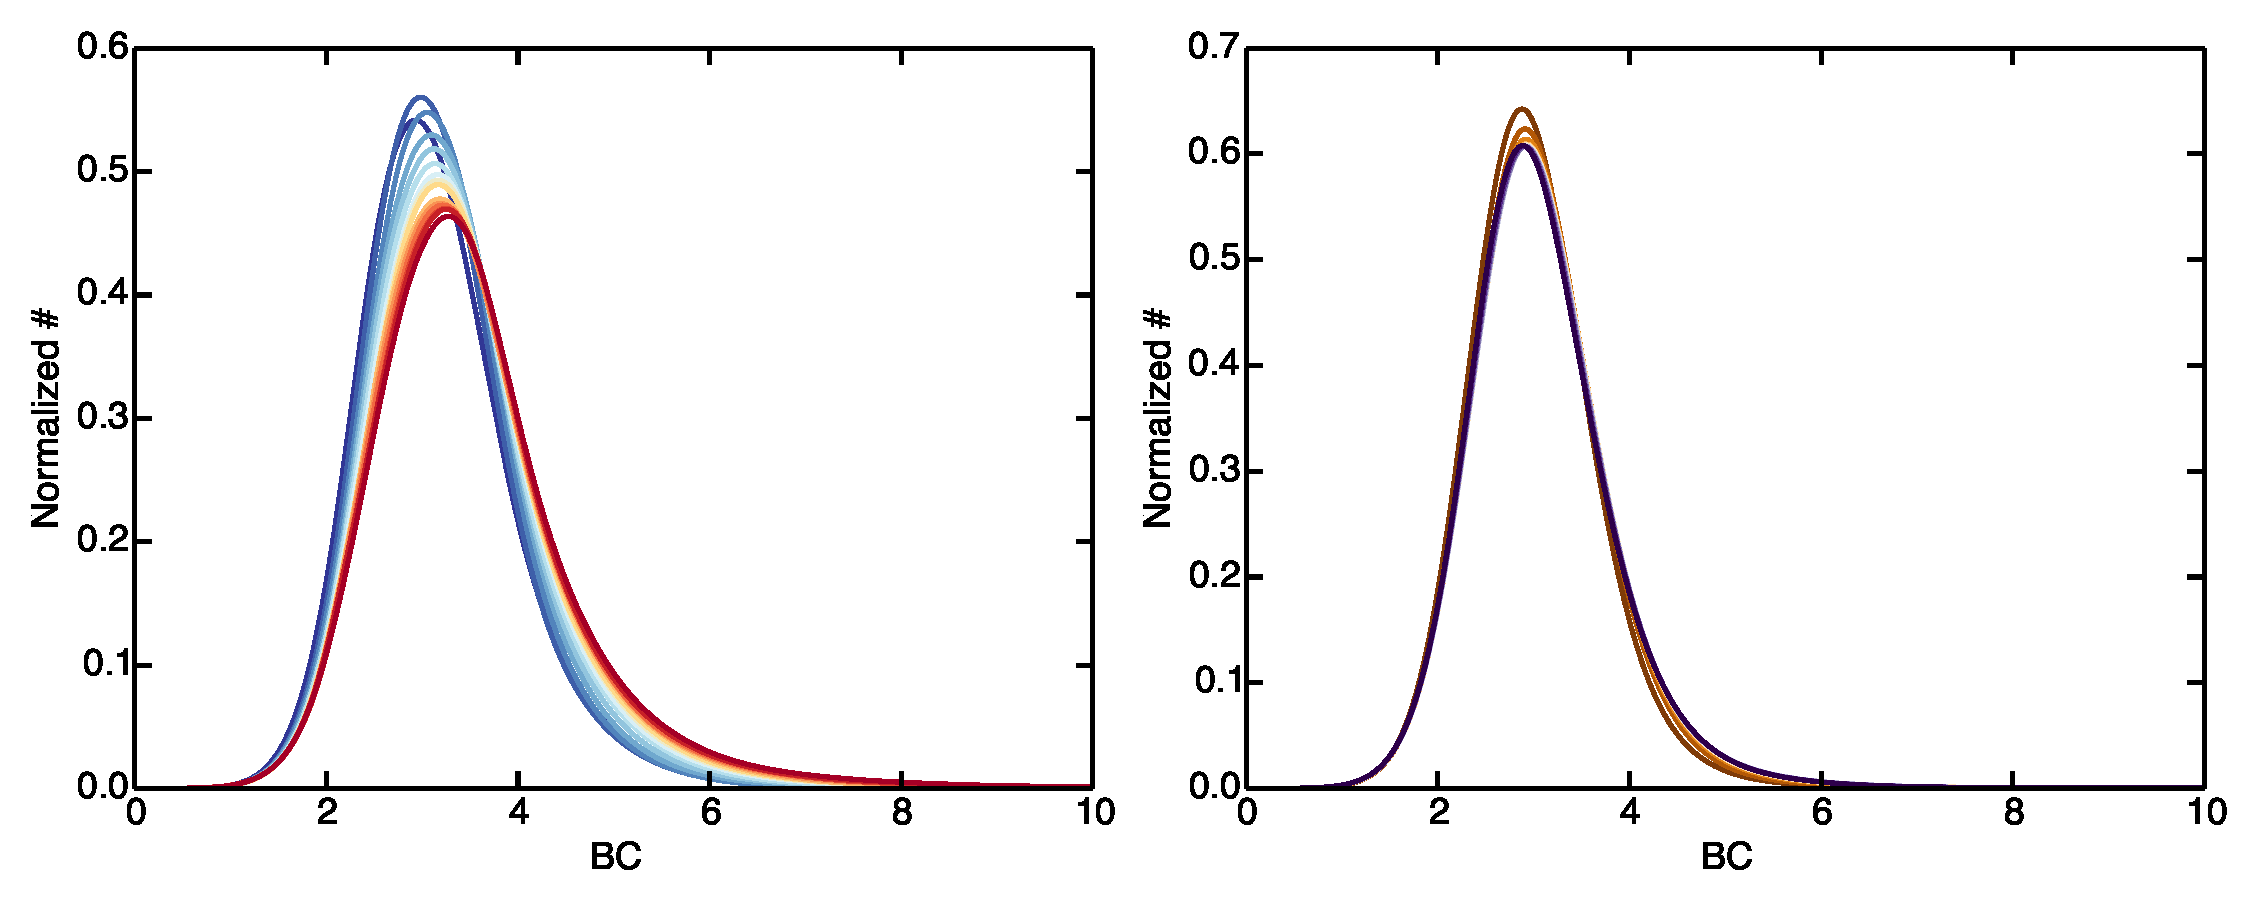
\includegraphics[width=5.5in]{images/BH/f8b} 
\end{tabular}
\begin{tabular}{cc}
	\hspace{.4cm} 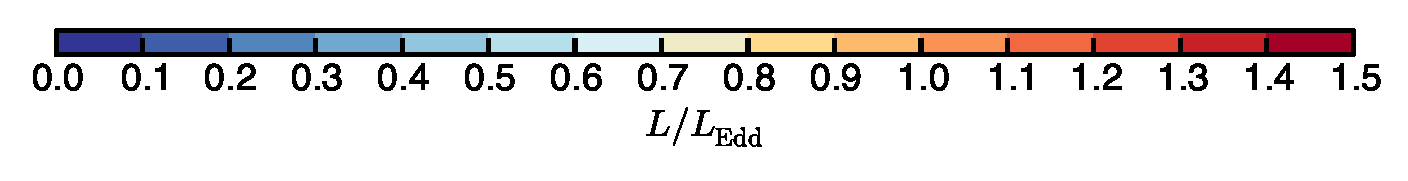
\includegraphics[width=2.5in]{images/BH/Lf_colorbar} & \hspace{.4cm} 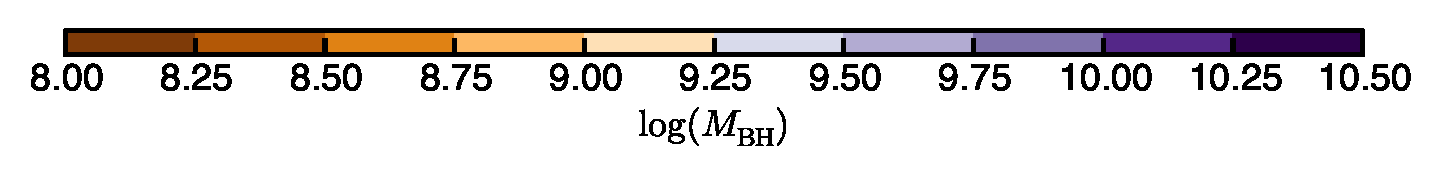
\includegraphics[width=2.5in]{images/BH/M_colorbar}
\end{tabular}
\caption[\ltwofive\ and \bctwofive\ distributions grouped by $\mbh$ and $\lf$]{\label{L_BC_mbh_lf} The fully marginalized \ltwofive\ ({\em top}) and \bctwofive\ ({\em bottom}) distributions grouped by common $\lf$ ({\em left}) and $\mbh$ ({\em right}). As expected both \ltwofive\ and \bctwofive\ and positively correlated with $\lf$.  There is a slight trend for higher $\mbh$ quasars to have higher \ltwofive, and there are no trends with \bctwofive.
%Both higher $\mbh$ and higher $\lf$ correlate with higher \ltwofive\ and higher \bctwofive.
}
\end{center}
\end{figure}

For our sample we used 10 bins in $\log{(\mbh)}$ (between 8--10.5) and 15 bins in $\lf$ (between 0--1.5).  The resulting SEDs grouped by $\lmbh$ are shown in Figure~\ref{Lfrac_sed} and the same SEDs grouped by $\lf$ are shown in Figure~\ref{Mbh_sed}. As expected, we see for a given $\lmbh$ bin the quasars with higher $\lf$ have more hot dust emission in the mid-IR and their BBB peaks at shorter wavelengths, both consistent with the accretion disk having a higher temperature.  We also note that the higher $\lmbh$ bins show an additional bump in the EUV.  This bump is highly dependent on the EUV extrapolation and gap-filling method used, and more work needs to be done to determine if this trend is real or just an artifact of our data analysis.
%possible evidence for more ionizing being present in these quasars.  However, we note that this is highly dependent on the EUV extrapolation method used, and more work needs to be done to determine if this trend is real or just an artifact of our data analysis. 
When grouping the quasars by $\lmbh$ we see a similar trend where more massive quasars are consistent with having a hotter accretion disk, the opposite trend that the $\alpha$-disk theory predicts.

%\subsection{The \ltwofive\ and \bctwofive\ Distributions}

Figure~\ref{L_BC_mbh_lf} shows the marginalized distributions for \ltwofive\ and \bctwofive\ based on $\lmbh$ and $\lf$ after picking sub-samples with common redshift distributions.  Both \bctwofive\ and $\lf$ are proportional to \lbol, so we expect these two values to be correlated, and $\lf$ to increase with luminosity.  Both of these trends are seen clearly in the data.  Looking at $\lmbh$ we see \ltwofive\ becomes slightly larger for more massive quasars and we find no significant changes in \bctwofive.
%we see that \ltwofive\ and \bctwofive\ both becomes larger for more massive quasars.  However, we do note that for both quantities the five most massive bins all have the same (normalized) distributions. This may be an indication of self-regulation within the quasar such that after the central black hole reaches $\sim10^{9} M_{\odot}$ the luminosity stops increasing [somehow related to the Eddington limit? Or it could be the result of a non-uniform redshift distribution.].

\section{Conclusions} \label{BH_conclusions}

Using the individual quasar's SEDs from Chapter~\ref{SEDs} and the extinction characterized in Chapter~\ref{Dust} we corrected the observed SEDs for dust reddening.  With these corrected SEDs we found trends with both intrinsic color and $\ebv$.  Bluer quasars show stronger emission around $3\,\mu$m and a shift in the minimum near $1\,\mu$m to shorter wavelengths (right panel of Figure~\ref{sed_dust_color_rc}), both evidence for stronger hot dust emission. These quasars also have their BBB peak further into the UV, indicative of a hotter accretion disk, and have a higher \bctwofive\ distribution (bottom right panel of Figure~\ref{L_BC_dust_color_rc}).  The shift in the BBB and increase in \bctwofive\ could also 
be explained if some of the blue quasars are actually intrinsically red, but are seen closer to edge-on, an explanation that helps to reconcile the weak ionizing lines seen in the composite spectra with the relatively hard SEDs seen in the EUV.
%large amounts of ionizing photons seen in the SEDs.
%Bluer quasars are consistent with have hotter accretion disks (right panel of Figure~\ref{sed_dust_color_rc}) and higher \bctwofive\ (bottom right panel of Figure~\ref{L_BC_dust_color_rc}).  These trends are also consistent with some of the blue quasars being intrinsically red, but seen edge-on, an explanation that helps to reconcile the weak ionizing lines seen in the composite spectra with the large amounts of ionizing photons seen the the SEDs.
%Although the quasar with more dust extinction have less hot dust, they do have more dust over all (left panel of Figure~\ref{sed_dust_color_rc}), higher luminosities, and smaller \bctwofive\ (left side of Figure~\ref{L_BC_dust_color_rc}).
We also find evidence for either an observational bias or intrinsic effect that changes the shape of the SED as a function of $\ebv$.  Although, it is unclear at this time what the cause of these changes are.
%Although we did not see any systematic trends in the SEDs with $\ebv$, quasars with larger $\ebv$ have lower luminosities and smaller \bctwofive\ (left side of Figure~\ref{L_BC_dust_color_rc}).

Using these corrected SEDs as a stepping stone, we constructed mean SEDs based on $\lmbh$ and $\lf$ (a proxy for accretion rate).
%Mean quasars SEDs based on $\lmbh$ and $\lf$ (a proxy for accretion rate) were also created. 
For a fixed $\lmbh$, quasars with larger $\lf$ were bluer, had BBB that peaked at shorter wavelengths, and more hot dust emission in the mid-IR.  All of these trends are expected from the $\alpha$-disk model where large $\lf$ corresponds with a hotter accretion disk.
%Quasars with larger $\lf$ were consistent with having hotter accretion disks; the trend expected from the $\alpha$-disk theory. 
If the $\alpha$-disk model is correct, we would expect to see the opposite trend as $\lmbh$ is increased and $\lf$ is fixed.  Instead, we see the same trends as we did with increasing $\lf$, indicating that the quasars with larger $\lmbh$ also have hotter accretion disks.
%Unexpectedly, the quasars with larger $\lmbh$ were also consistent with having hotter accretion disk.  
These large $\lmbh$ SEDs also show an additional bump in the EUV, but it is unclear if this trend is real or an artifact of our data analysis.
%indicating they have more ionizing radiation than lower mass quasars.  
As expected, we found quasars with large $\lf$ also had higher luminosities and larger \bctwofive.  There was also a slight trend with higher mass quasars also having higher luminosities, but no trend was found between $\lmbh$ and \bctwofive.
%Looking at the \ltwofive\ and \bctwofive\ distributions, the quasars with larger $\lf$ had larger \ltwofive\ and \bctwofive, while the quasars with larger $\lmbh$ only had slightly larger \ltwofive\ and no trend in \bctwofive.